\documentclass[12pt,a4paper]{report}

%Set language
\usepackage[english]{babel}
\usepackage{enumerate}

% To import and adjust images
\usepackage{graphicx}
\usepackage[export]{adjustbox}
\usepackage[center]{caption}
\usepackage{subcaption}
\usepackage{float}
\usepackage{tabularx}

% To build a clickable Toc
\usepackage{color}   %May be necessary if you want to color links
\usepackage{hyperref}
\hypersetup{
    colorlinks=true, %set true if you want colored links
    linktoc=all,     %set to all if you want both sections and subsections linked
    linkcolor=black,  %choose some color if you want links to stand out
    urlcolor = black
}

%To load PoLitecnico's logo
\usepackage{titling}

% Command to hide subsections in the Toc
\setcounter{tocdepth}{1}

% I don't like dots in the Toc
\usepackage{tocloft}
\renewcommand{\cftdot}{}

% To import alloy source code
\usepackage[dvipsnames]{xcolor}
\usepackage{listings}
\usepackage{alloy-style}

% Path relative to the .tex file containing the \includegraphics command
\graphicspath{ {./images/} }  

% To change the ToC title
\addto\captionsenglish{ \renewcommand {\contentsname} {Table of contents}}

%logo 
\pretitle{
	 \begin{center}
	 \LARGE
	 
\includegraphics[width = 0.6\textwidth]{logo}\\[\bigskipamount]
}
\posttitle{\end{center}}

% Here we go
\title{SafeStreets - RASD \\ \large version 1.0}
\author{Frangi Alberto, Fucci Tiziano}
\date{A.Y. 2019/2020}
\begin{document}
\maketitle

% Index
\tableofcontents
\chapter{Introduction}
	\section{Purpose}
SafeStreets is a crowd-sourced application that intends to allow users to notify authorities when traffic violations occur, and in particular parking violations, such as vehicles parked in the middle of bike lanes or in places reserved for people with disabilities, double parking, and so on. The application allows users to send pictures of violations, including their date, time, and position, to authorities.
 
SafeStreets stores the information provided by users, completing it with suitable meta-data. In particular, when it receives a picture, it runs an algorithm to read the license plate (one can also think of mechanisms with which the user can help with the recognition), and stores the retrieved information with the violation, including also the type of the violation (input by the user) and the name of the street where the violation occurred (which can be retrieved from the geographical position of the violation). 

The application allows both users and authorities to mine the information that has been received, for example by highlighting the streets (or the areas) with the highest frequency of violations, or the vehicles that commit the most violations. 

Moreover, if the municipality offers a service that allows users to retrieve the information about the accidents that occur on the territory of the municipality, SafeStrees can cross this information with its own data to identify potentially unsafe areas, and suggest possible interventions (e.g., add a barrier between the bike lane and the part of the road for motorized vehicles to prevent unsafe parking).


	\section{Scope}
	\subsection{General description}
Safestreet is an application to be used both from civilians (users) and authorities, in order to help the latter and reduce traffic violations. Registered authorities can automatically receive reports made by users, so the service acts as an intermediary. The next paragraph gives a more formal description of which is the purpose of the application.

	\subsection{Goals}
	The following list describes the goals from the S2B perspective:
		\subsubsection{User}
	% Dot list 
	\begin{itemize}
		\item \textbf{G1}: The application must allow the users to register entering an e-mail address and a password.
		\item \textbf{G2}: The application must allow the users to notify traffic violations, providing  the type of violation and a picture of the vehicle.
		\item \textbf{G3}: The application must be able to show to the users the streets and the vehicles with the highest frequency of violations.
		\item \textbf{G4}: The application must allow the users to see all of their reports and their status.
		\item \textbf{G5}: The application must notify the users when one of their reports is evaluated.
	\end{itemize}
		\subsubsection{Authority}
	\begin{itemize}
		\item \textbf{G6}: The application must allow the authorities to register providing a valid identification number and a valid password.
	  	\item \textbf{G7}: The application must allow the authorities to retrieve and evaluate the available reports.
		\item \textbf{G8}: The application must be able to identify potentially unsafe areas and suggest possible interventions.
	\end{itemize}
	

	\section{Definitions, acronyms, abbreviations}
		\subsection{Definitions}
		\begin{itemize}
		\item \textbf{User}: a civilian customer that can use the application to:
			\begin{itemize}
			\item notify authorities of some violation;
			\item check which are the most dangerous (i.e. with the most violations) streets;
			\end{itemize}
		in this document, ``user", ``citizen" and ``civiian" are completely equivalent, where not specified.
		\item \textbf{Authority}: a member of the local police who has access to reports made by users. The 					authorities evaluate the reports sent by the user to determine if the violation stands.
		\item \textbf{Report}: a message consisting of:
			\begin{itemize}
			\item a picture showing the car in order to show the occurring violation;
			\item date and time of the picture;
			\item GPS position of the place where the violation occurred;
			\item the street where the violation occurred (automatically retrieved from the geographical position);
			\item the type of the violation (input by the user)
			\end{itemize}
		\item \textbf{Available}: a report is available for an authority if its position is within the municipality assigned to the authority.
		\item \textbf{Violation}: a situation that, according to the user who sent the report, is a violation of the traffic laws.
		\item \textbf{Intervention}: a brief text suggesting a possible solution in order to improve safety and discourage future violations.
		\end{itemize}
		\subsection{Acronyms}
			\begin{itemize}
			\item \textbf{API}: \emph{Application Programming Interface.}
			\item \textbf{GPS}: \emph{Global Positioning System.}
			\item \textbf{UI}: \emph{User Interface.}		
			\item \textbf{S2B}: \emph{Software-to-be.}				
			\item \textbf{PKC}: \emph{Public Key Cryptography.}		
			\item \textbf{AES}: \emph{Advanced Encryption Standard.}		
			\end{itemize}

	\section{Reference documents}
	The main reference document is the ``SafeStreets Mandatory Project Assignment'' specification document. The complete list of references is provided in chapter 6.

	\section{Document structure}
	\begin{itemize}
	\item \textbf{Chapter 1} is an introduction: it presents the document and the S2B with its scope and goals. It also helps the reader to understand, by giving the necessary definitions and explaining acronyms and abbreviations; 
	\item \textbf{Chapter 2} is a summary description of all the project. It gives a general idea of how the application works and shows the assumpions made in the development;
	\item \textbf{Chapter 3} presents the requirements to be guaranteed in order to achieve every goal of the project, analyzing every use case. It shows the constraints and the attributes of the system in terms of availability, mantainability, secturity etc.;
	\item \textbf{Chapter 4} contains the Alloy model of critical aspects that require special attention. Here it is shown how the project has been modeled and a proof of the model consistency is provided. Moreover, examples of some of the generated world are shown;
	\item \textbf{Chapter 5} is meant to show how work was divided between the two components of the group and how much time was spent;
	\item \textbf{Chapter 6} lists the reference documents and the tools used to develop this document.
	\end{itemize}

% End of first chapter

\chapter{Overall description}
	\section{Product perspective}
		SafeStreets wants to be a mediator between authorities and citizens, allowing the last ones to report traffic violations, see which zone has the highest number of violations, see the recap of all the previous reports and their state
		(seen, approved, rejected, in queue). In order to be able to report various violations a user has firstly to be in a
		territory covered by any authority who has signed up to SafeStreets, and has to sign up providing his e-mail address, unique for each user. Any authority has to verify its identity using the institutional email address.
		To avoid spamming of requests, pending reports will be put in a priority queue based 
		on a reliability index associated to each user and hidden to both side of communication (it is an information used only by 
		the system for the priority queue). If the authorities evaluates a violation, the user who has reported it
		will receive a notification by SafeStreets, to inform him of the success (or failure) of his report. 
		\begin{figure}[H]
			\begin{subfigure}{\textwidth}
				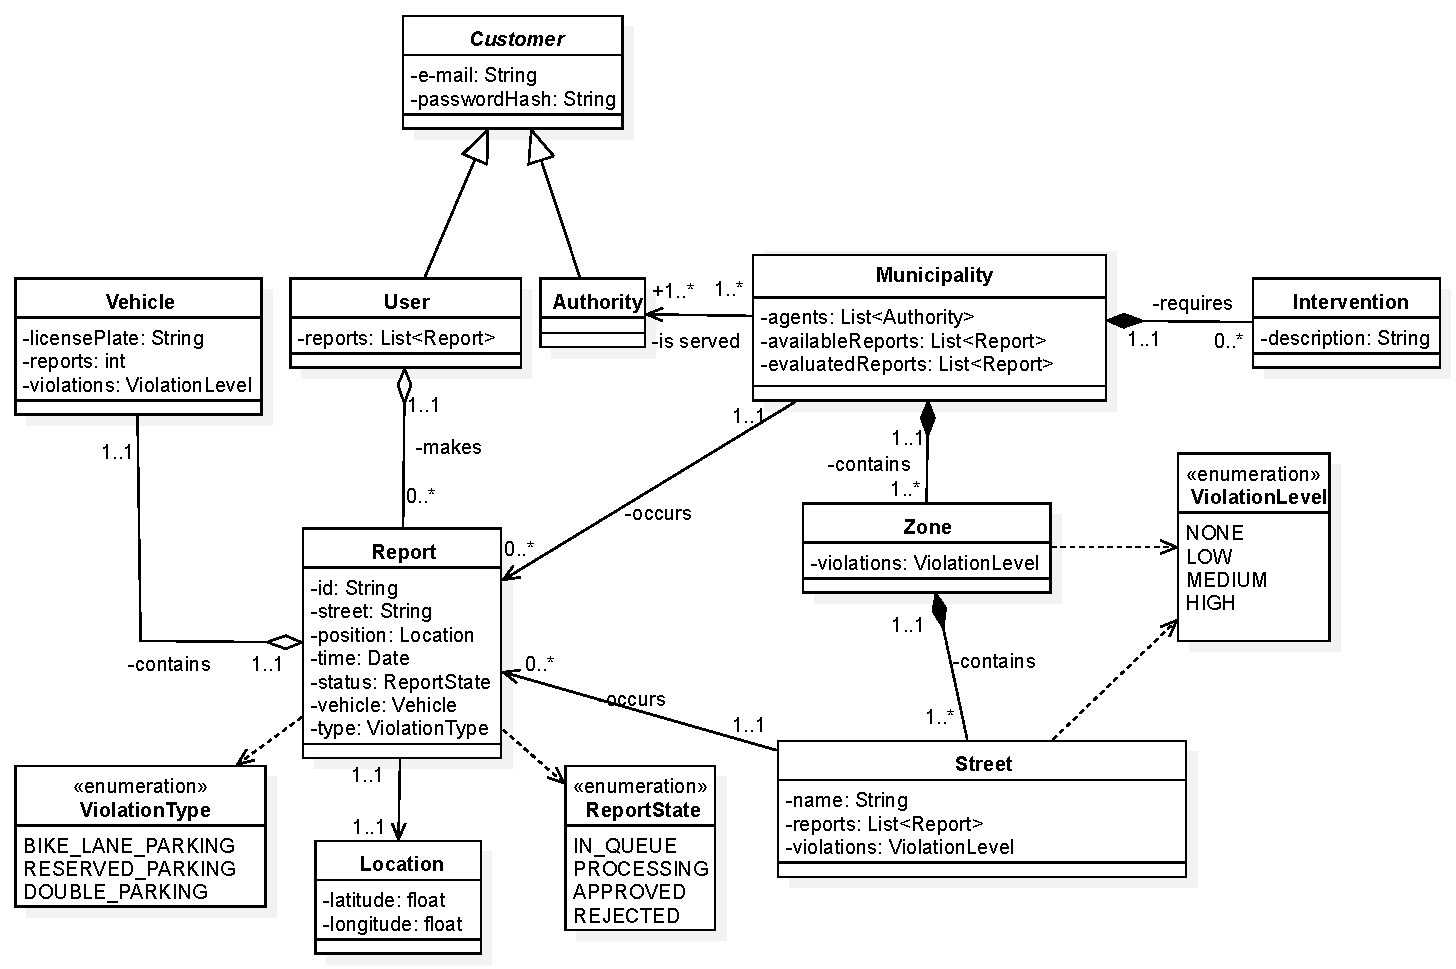
\includegraphics[scale = 0.65, center]{uml}
				\caption{UML model}
				\label{UML model }
			\end{subfigure}
		\end{figure}
		This figure represents a draft of how the system's UML model will be. Since it is only the model part, the represented classes are only the few essential to save correctly all the data necessary for the analysis. In order to save up space it has been avoided to write every single getter and setter or attribute.
		A generic Customer has been modeled with an abstract class and both authorities and user inherit it.
		Report is a combination of various classes, it contains a unique id, the Street (obtained by the GPS position), the time (obtained
		by the system when it receives the report), the vehicle license's plate and the type of violation, it also has an enum attribute
		to represent the status of the report. Both ``Street" and ``Zone" (which is a set of streets) contain a ViolationLevel, that
		is calculated by the system and based on the number of reports in that particular street/zone. An Intervention is a suggestion made
		by the system to improve security, it is chosen by a recommender system that applies some simple data mining's algorithms
		in order to find the best improvement for each street, based on the most frequent violations or accidents.
		Municipality contains a list of possible interventions, all the authorities that operate in its territory and all reports
		(both evaluated and to evaluate).

		Now some critical aspects of the application will be analyzed, modeling their behaviors and	
		showing the evolution over time of their	states through appropriate state diagrams, which are
		reported below.
		
		\begin{figure}[H]
			\begin{subfigure}{\textwidth}
				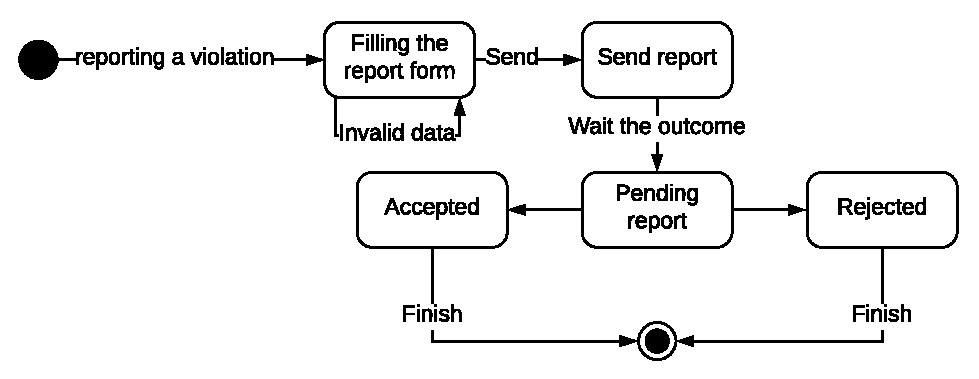
\includegraphics[scale = 0.75, center]{reportC}
				\caption{State diagram on the behavior of reports for users}
			\end{subfigure}
		\end{figure}
		This diagrams represent the behavior of the reporting system (for the citizen). The concept is pretty straight forward: the system does not allow to send reports
		with missing information or with wrong ones.
		
		\begin{figure}[H]
			\begin{subfigure}{\textwidth}
				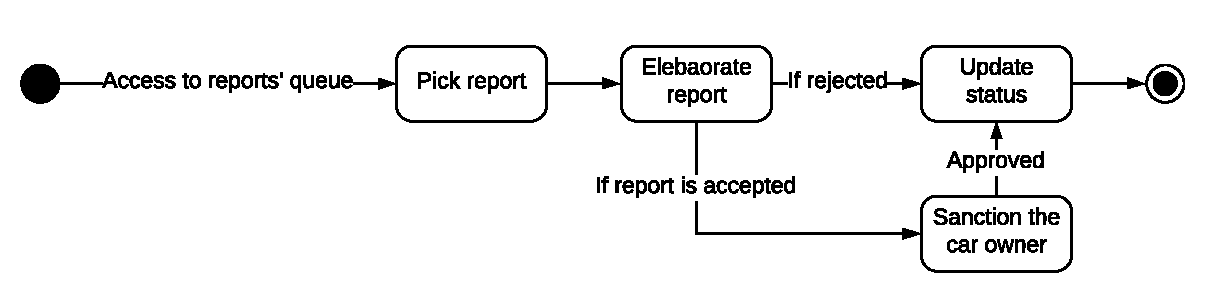
\includegraphics[scale = 0.75, center]{reportA}
				\caption{State diagram on how reports work for authorities}
			\end{subfigure}
		\end{figure}	
		This diagram is inherent to the reports verification process,
		it shows the evolution of the states necessary to handle a report, from when the authorities take in charge a user's report
		to the eventual sanction to the car owner. A sanction will result in the car being noticed, incrementing its reports' number. In the long run, this can take to increasing the violation level of that vehicle.
		
		\begin{figure}[H]
			\begin{subfigure}{\textwidth}
				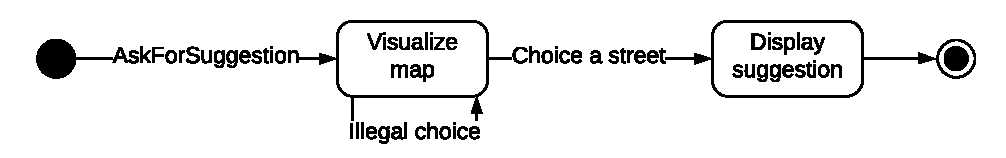
\includegraphics[scale = 0.75, center]{suggestion}
				\caption{State diagram on how reports work for authorities}
			\end{subfigure}
		\end{figure}
		This last diagram represents the last major functionality offered by SafeStreet. It consists in a system that offers suggestions
		on how improve safety on particular streets, based on the occurrences of car accidents and street violations data that
		the authorities choose to share with SafeStreets.
		  
		
	\section{Product functions}
		In the following section the most important product functions of the system are reported.
		Safe Streets offers to its users the possibility to report traffic violations, check the status of the previous reports and see 
		a map that indicates the areas with the highest number of reports verified.
		\subsection{Report}
			To report a violation a user has to take a picture of the possible violation with the plate visible, choose what type of
			violation it is from various possible categories and send the position.
		\subsection{Status}
			This functionality allows user to see a recap of all the reports they have made. The information that will be displayed
			are: date and time, place, type of violation and status. The last one can be:
			\begin{itemize}
				\item \textbf{In queue:}
					in this status the report is waiting to be analyzed by an authority. The report's priority is based on
					the user who created it. All the users, at the moment of the registration, have a standard value, that can increase or decrease basing on	how Safe Street is used. Some important factors are, for example, 
					how many reports a user sent has been rejected, how many reports a user sent can decrease
					the priority, but a wisely use of the system can increase it, like a streak of approved reports.
				\item \textbf{Processing:}
					in this status the authorities has seen the report and are considering the violation and if it is a real
					violation.
				\item \textbf{Approved:}
					the report has been seen by authorities and the violation has been recognized and sanctioned. 
				\item \textbf{Rejected:}
					the report has been seen by authorities and the violation hasn't been recognized.
			\end{itemize}
		\subsection{Map}
			This function allows the user to open the map and see the ``level of violations" of the different areas. These ``levels" are
			based on how many reports have been approved in that area: higher the level, higher the number of violation.
			There are 4 levels, which are indicated with different color, from no colour (level 0) to red (level 3).
			
	\section{User characteristics}
		The actors of the application are the following:
		\begin{itemize}
			\item \textbf{User:}
				a civilian who has registered to SafeStreets. He doesn't need any particular skill to use the system, 
				he is just supposed to have a smartphone (or tablet) with a functioning camera, an internet connection and
				a phone that can send its current position.  To make a report it is sufficient to
				take a picutre of the license plate, the violation's type and the system retrieves autonomously the current position
				of the user.
			\item \textbf{Authority:}
				An agent of the local police of a certain municipality exploiting SafeStreets, that has access to all the reports made
				 in his municipality. The authority can visualize the available reports and evaluate them, that is telling if the
				violation reported by the user stands or it is not a proper violation. After seeing a report, the authority 
				changes its status to Approved or Rejected. By activateing
				an optional service, authorities can check the streets with the highest number of accidents and receive
				suggestions (chosen by the system) to improve safety.
		\end{itemize}
	\section{Assumptions, dependencies and constraints}
	\subsection{Domain assumption} 
The following are the assumptions made to simplify and clarify some situation that could uselessly complicate the development of the application. Notice that some trivial assumptions are not included, in order to avoid their repetition in every situation (e.g. ``The devices always work without failure").
		\begin{itemize}
			\item \textbf{D1}: The users always provide a picture that allows both the algorithm to read the license plate and
					        the authority to identify the violation.
			\item \textbf{D2}: Every user is provided with a device capable to share the exact GPS position at any moment.
			\item \textbf{D3}: The name of the street where a violation occured is retrieved from the GPS position.
			\item \textbf{D4}: Authorities never make mistakes in evaluating a report.
			\item \textbf{D5}: Reports are evaluated only one time.
			\item \textbf{D6}: The user sends the report staying in the same place of the violation.
			\item \textbf{D7}: The picture of the license plate is taken at the moment and shows the right car.
		\end{itemize}


% End of second chapter

\chapter{Specific Requirments}
	\section{External interface requirments}
		\subsection{User interfaces}
		In this section some screenshots from the user interface are shown.
		\begin{figure}[H]
		\begin{subfigure}{0.5\textwidth}
			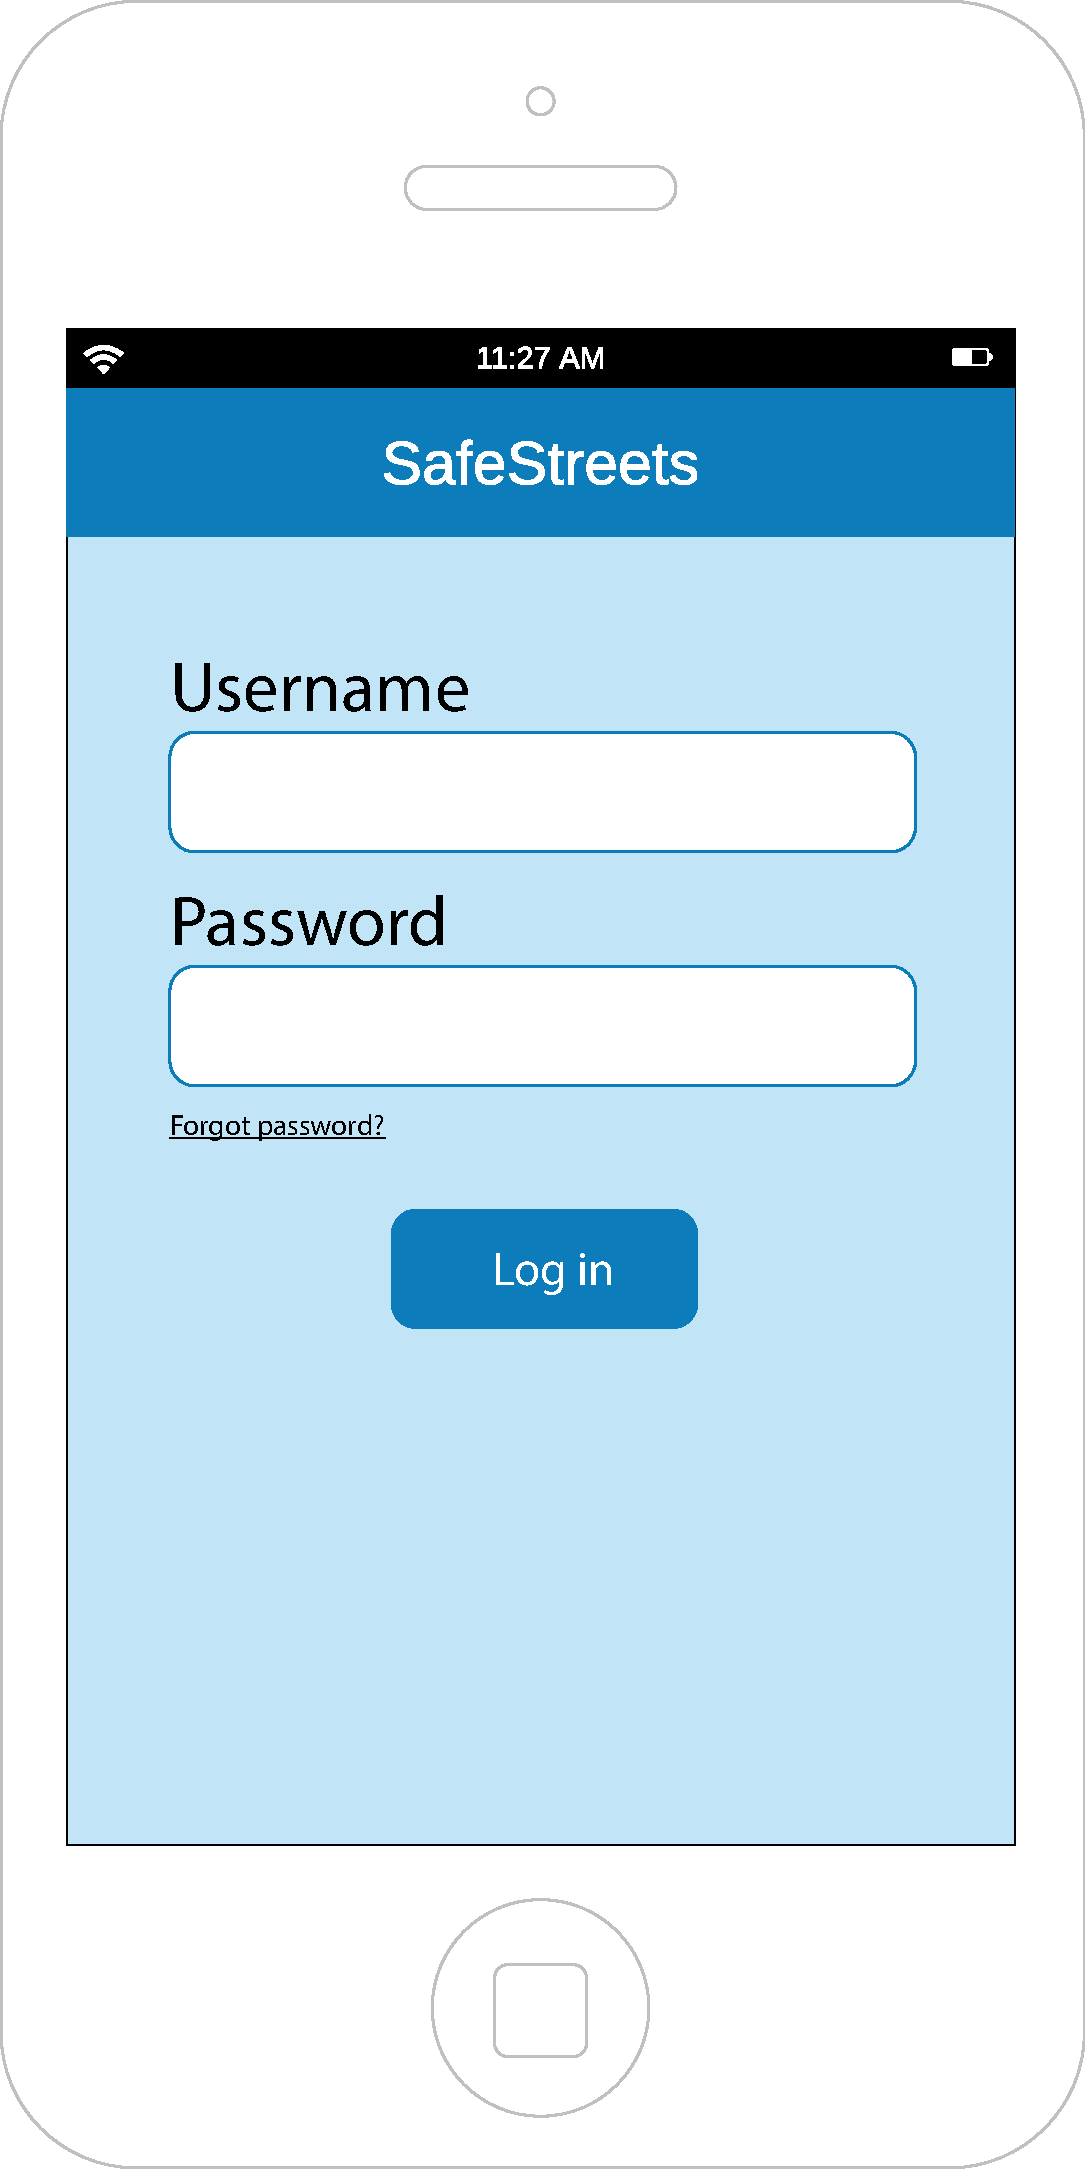
\includegraphics[scale=0.25, center]{Login}
			\caption{User - login}
			\label{Login}
		\end{subfigure}
		\begin{subfigure}{0.5\textwidth}
			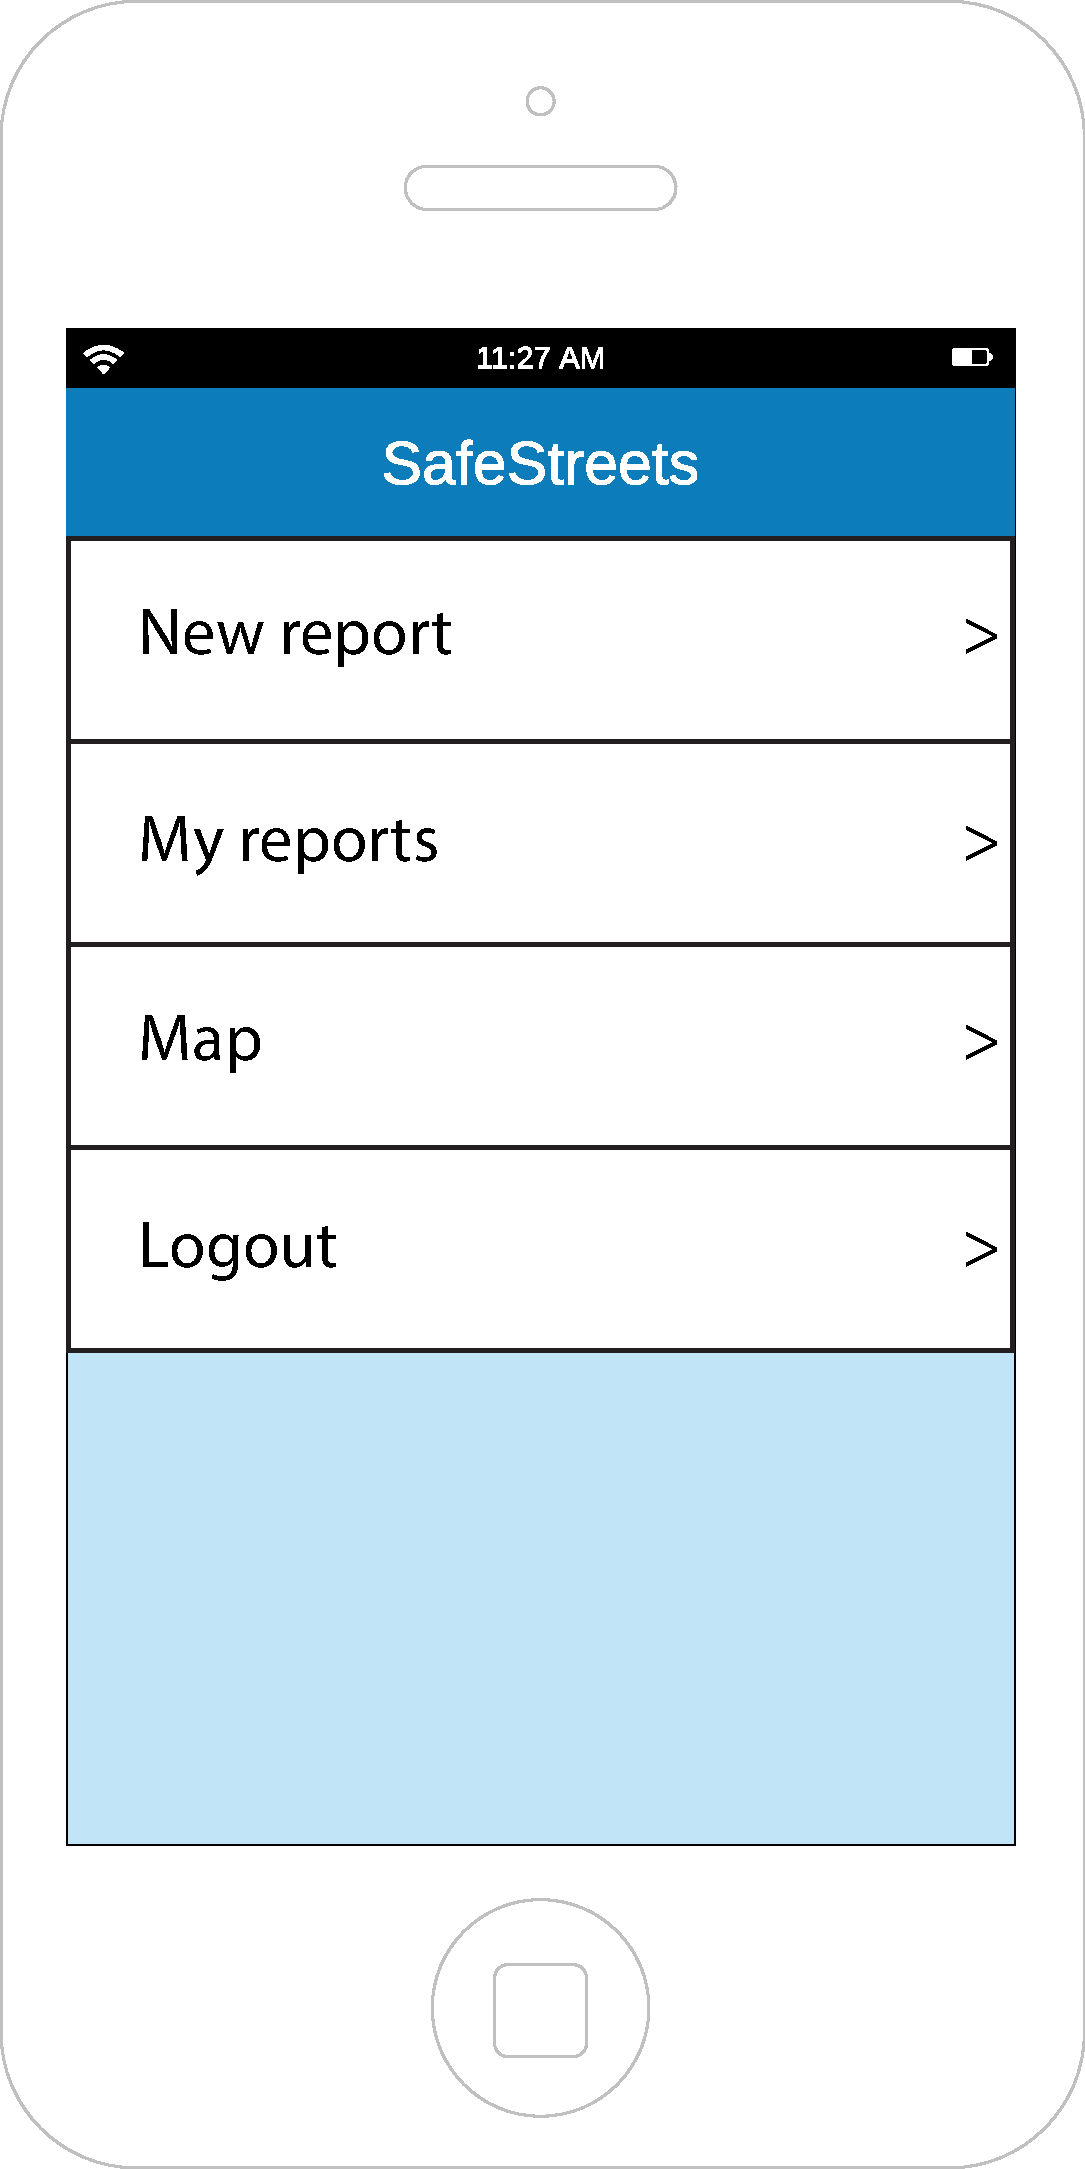
\includegraphics[scale=0.25, center]{Home}
			\caption{User - home}
			\label{Home}
		\end{subfigure}
		\end{figure}

		\begin{figure}[H]
		\begin{subfigure}{0.5\textwidth}
		\setcounter{subfigure}{2}
			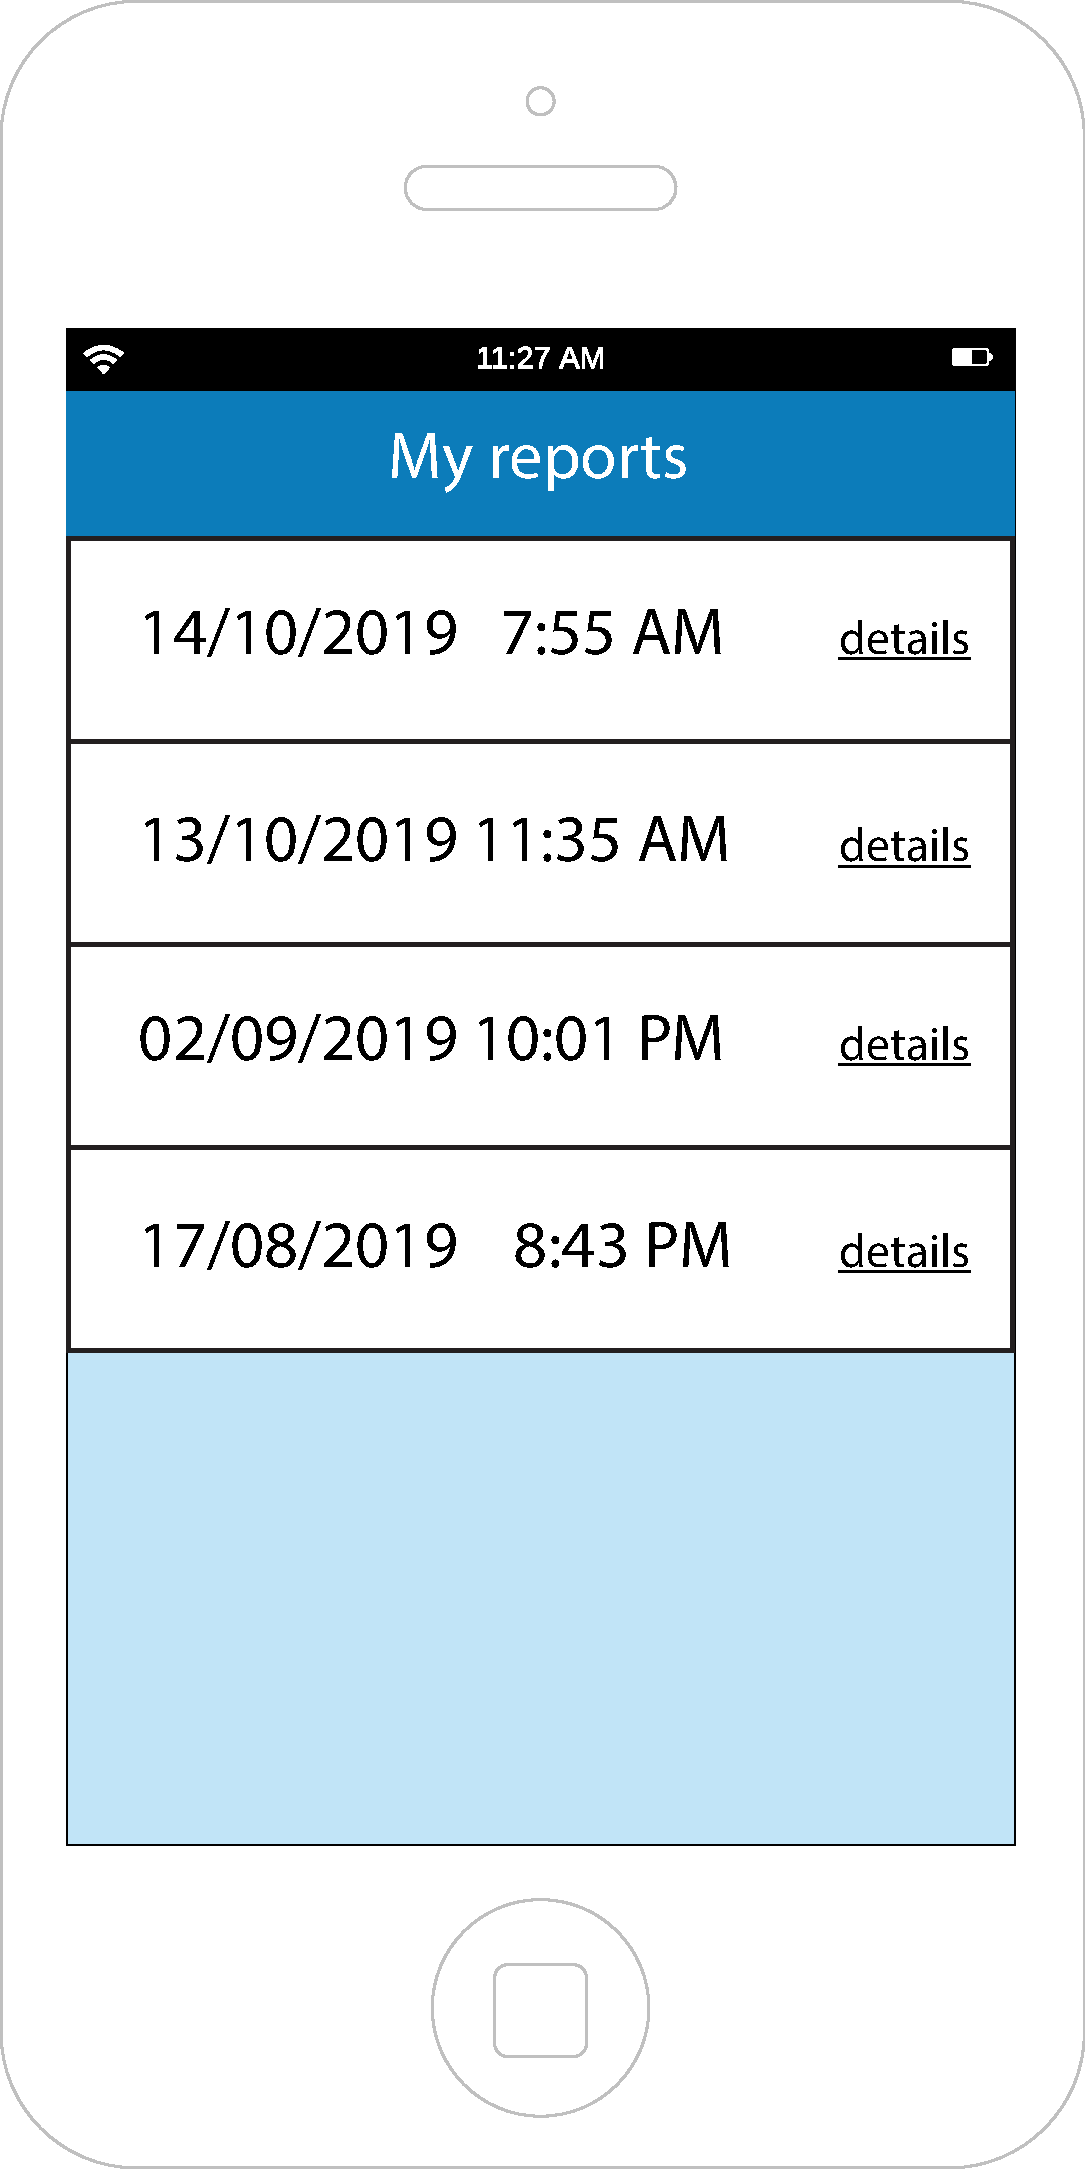
\includegraphics[scale=0.25, center]{Myreports}
			\caption{User -  list of sent reports}
			\label{List of sent reports}
		\end{subfigure}
		\begin{subfigure}{0.5\textwidth}
			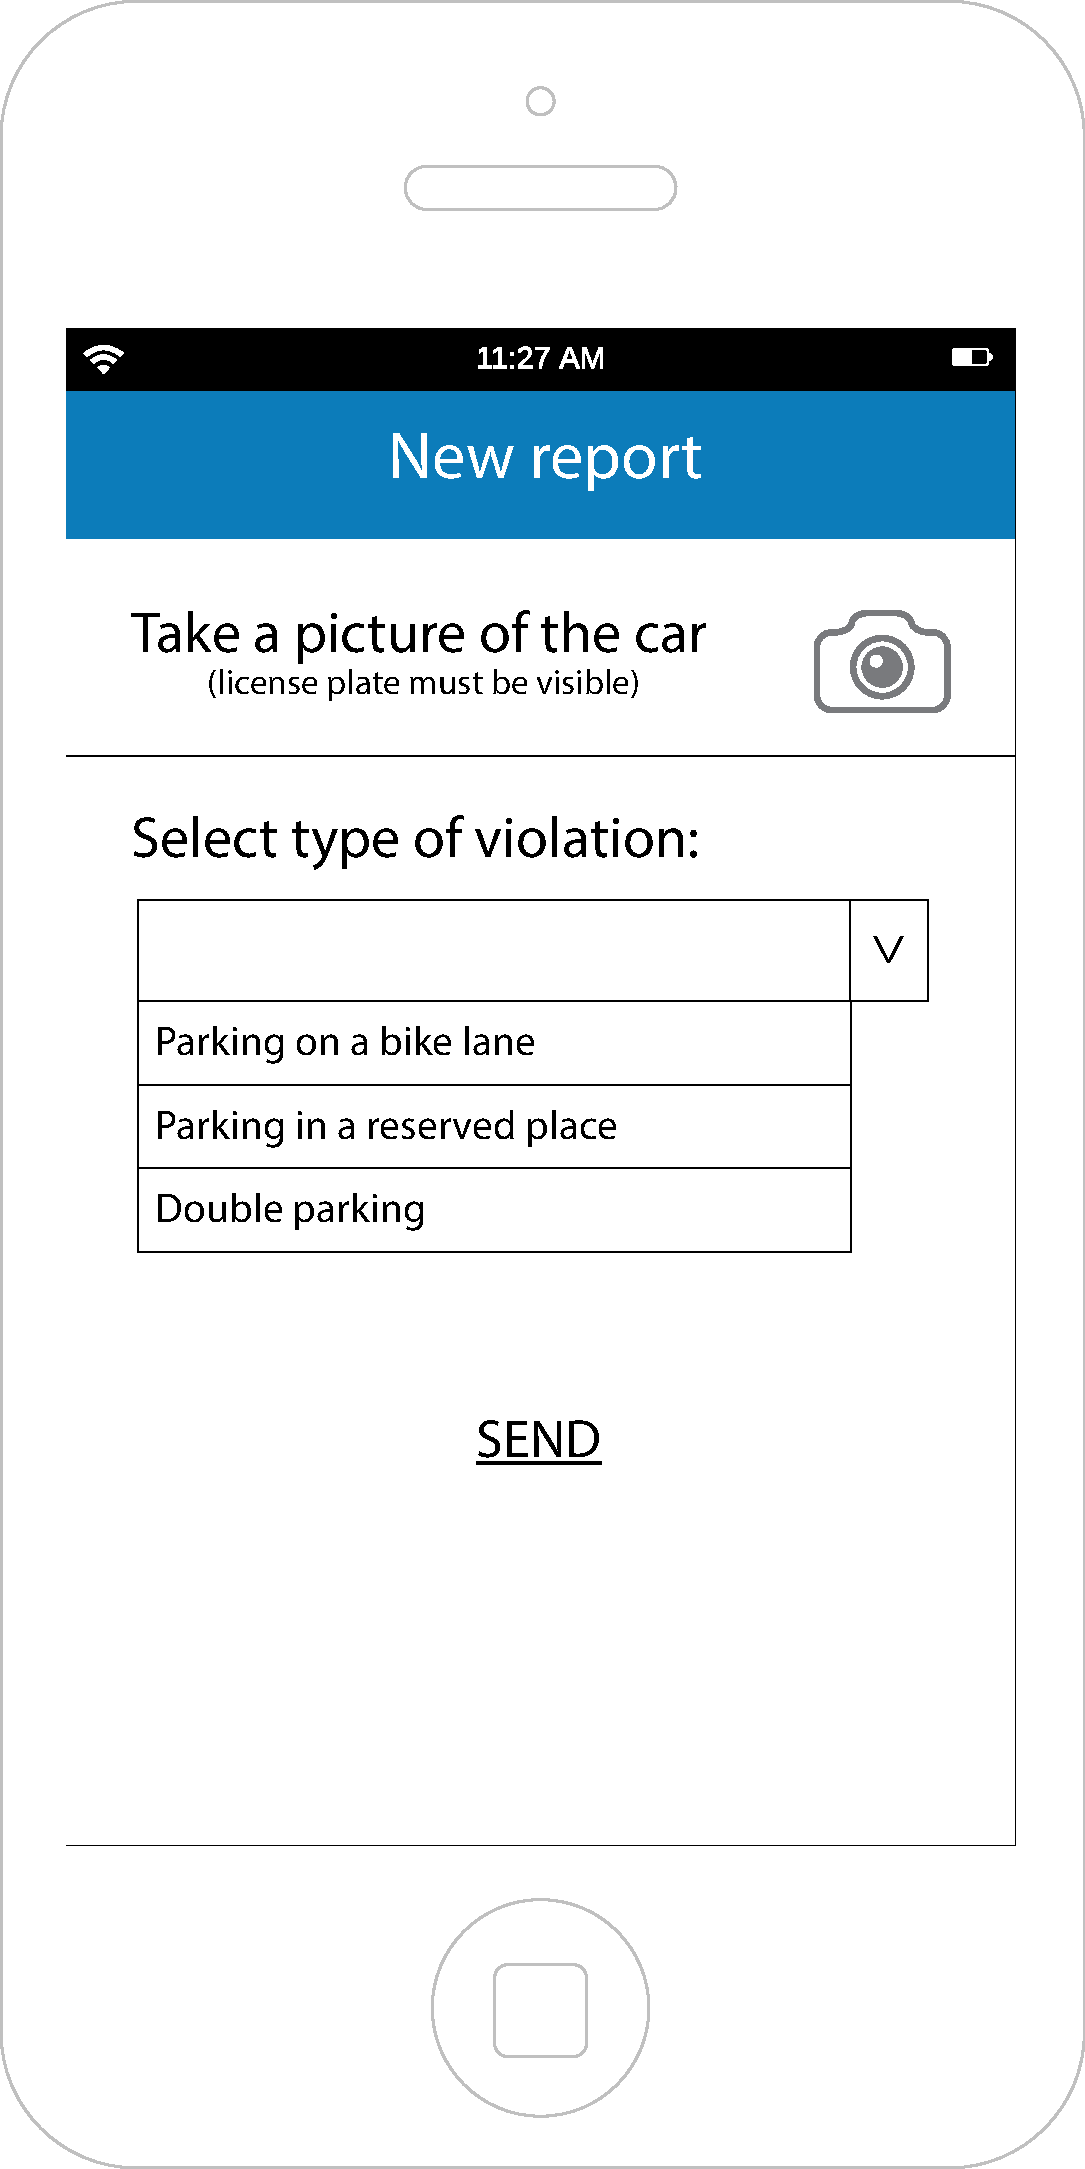
\includegraphics[scale=0.25, center]{Newreport}
			\caption{User -  new report}
			\label{fig:subim2}
		\end{subfigure}
		\end{figure}

		\begin{figure}[H]
		\begin{subfigure}{0.5\textwidth}
		\setcounter{subfigure}{4}
			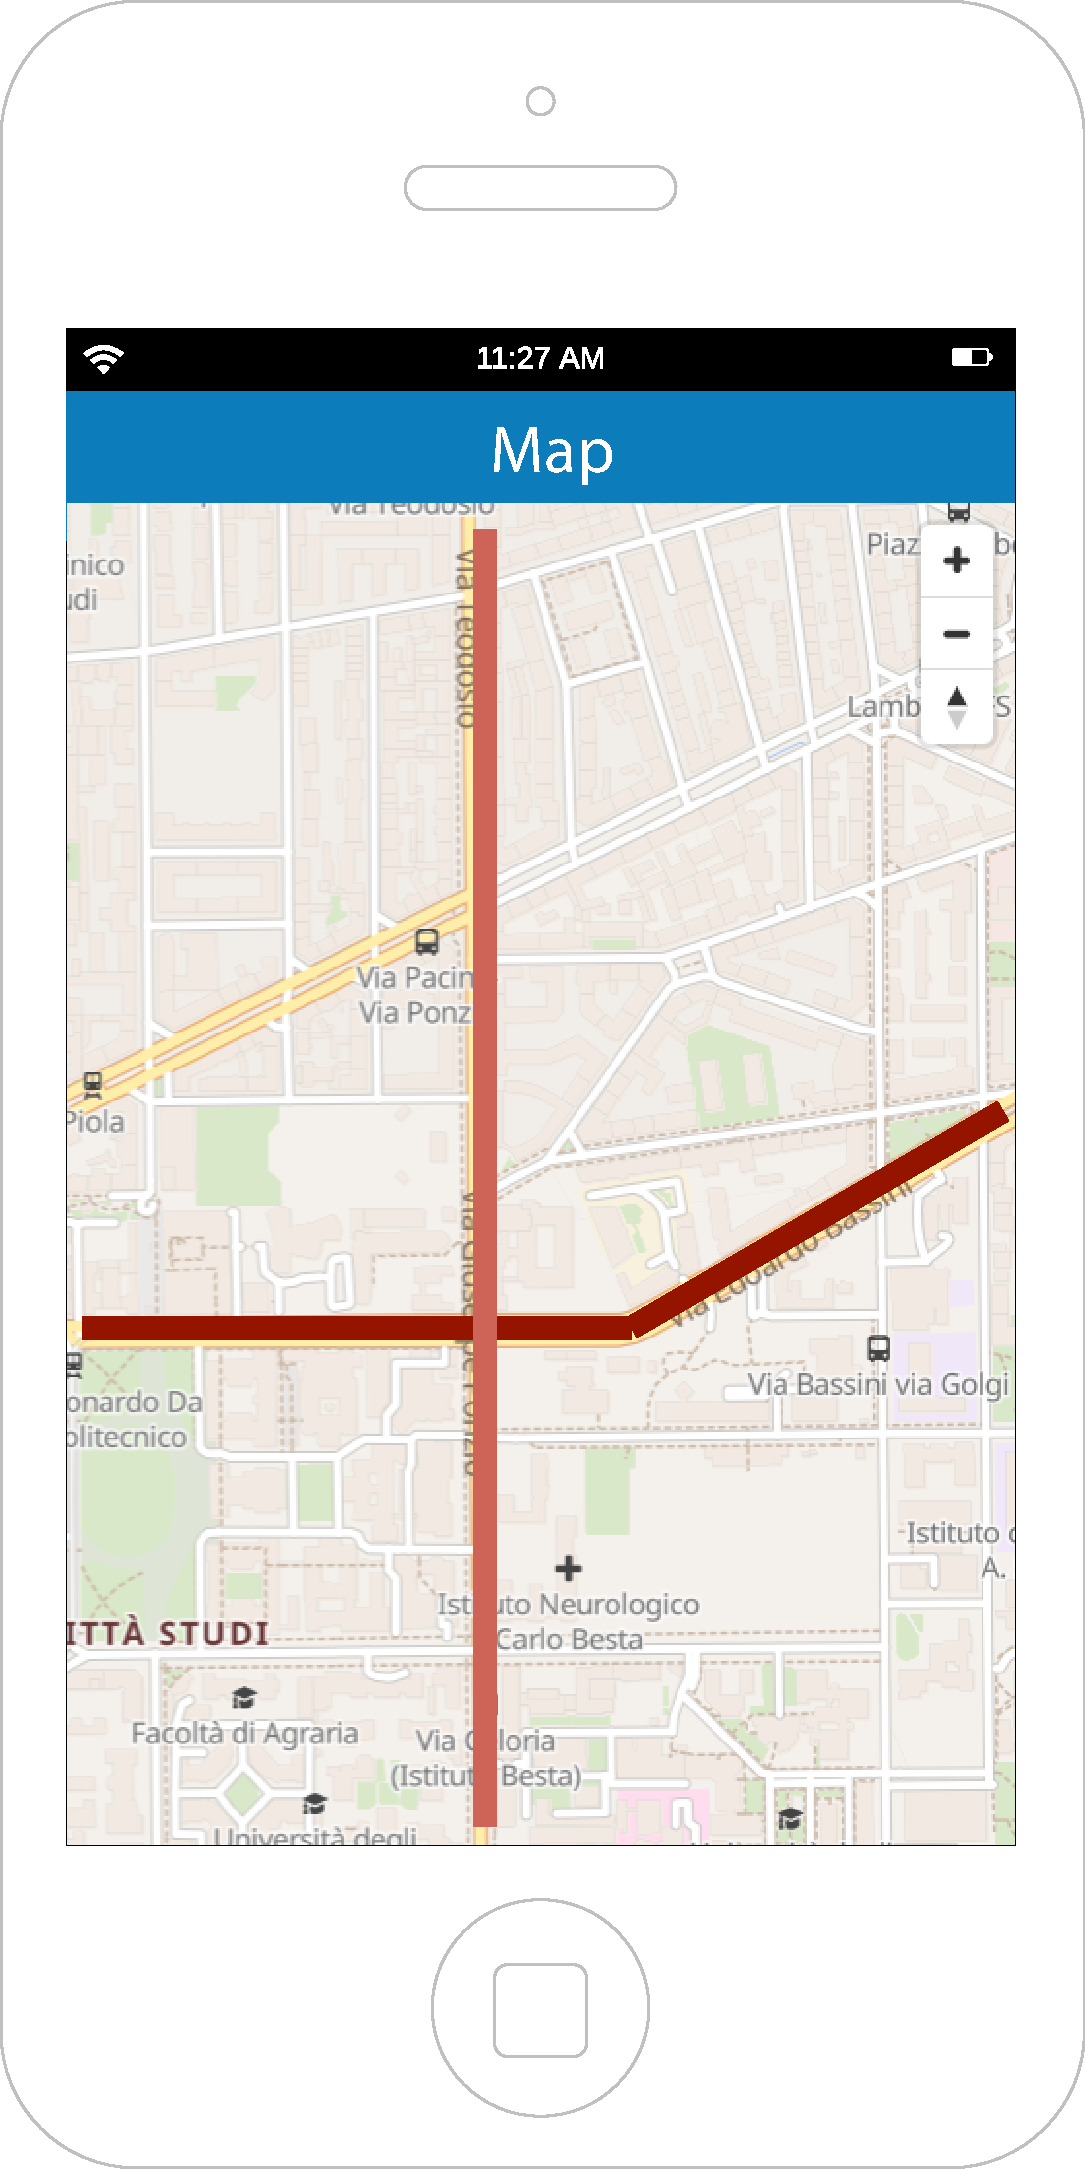
\includegraphics[scale=0.25, center]{Map}
			\caption{User -  map}
			\label{fig:subim2}
		\end{subfigure}
		\begin{subfigure}{0.5\textwidth}
			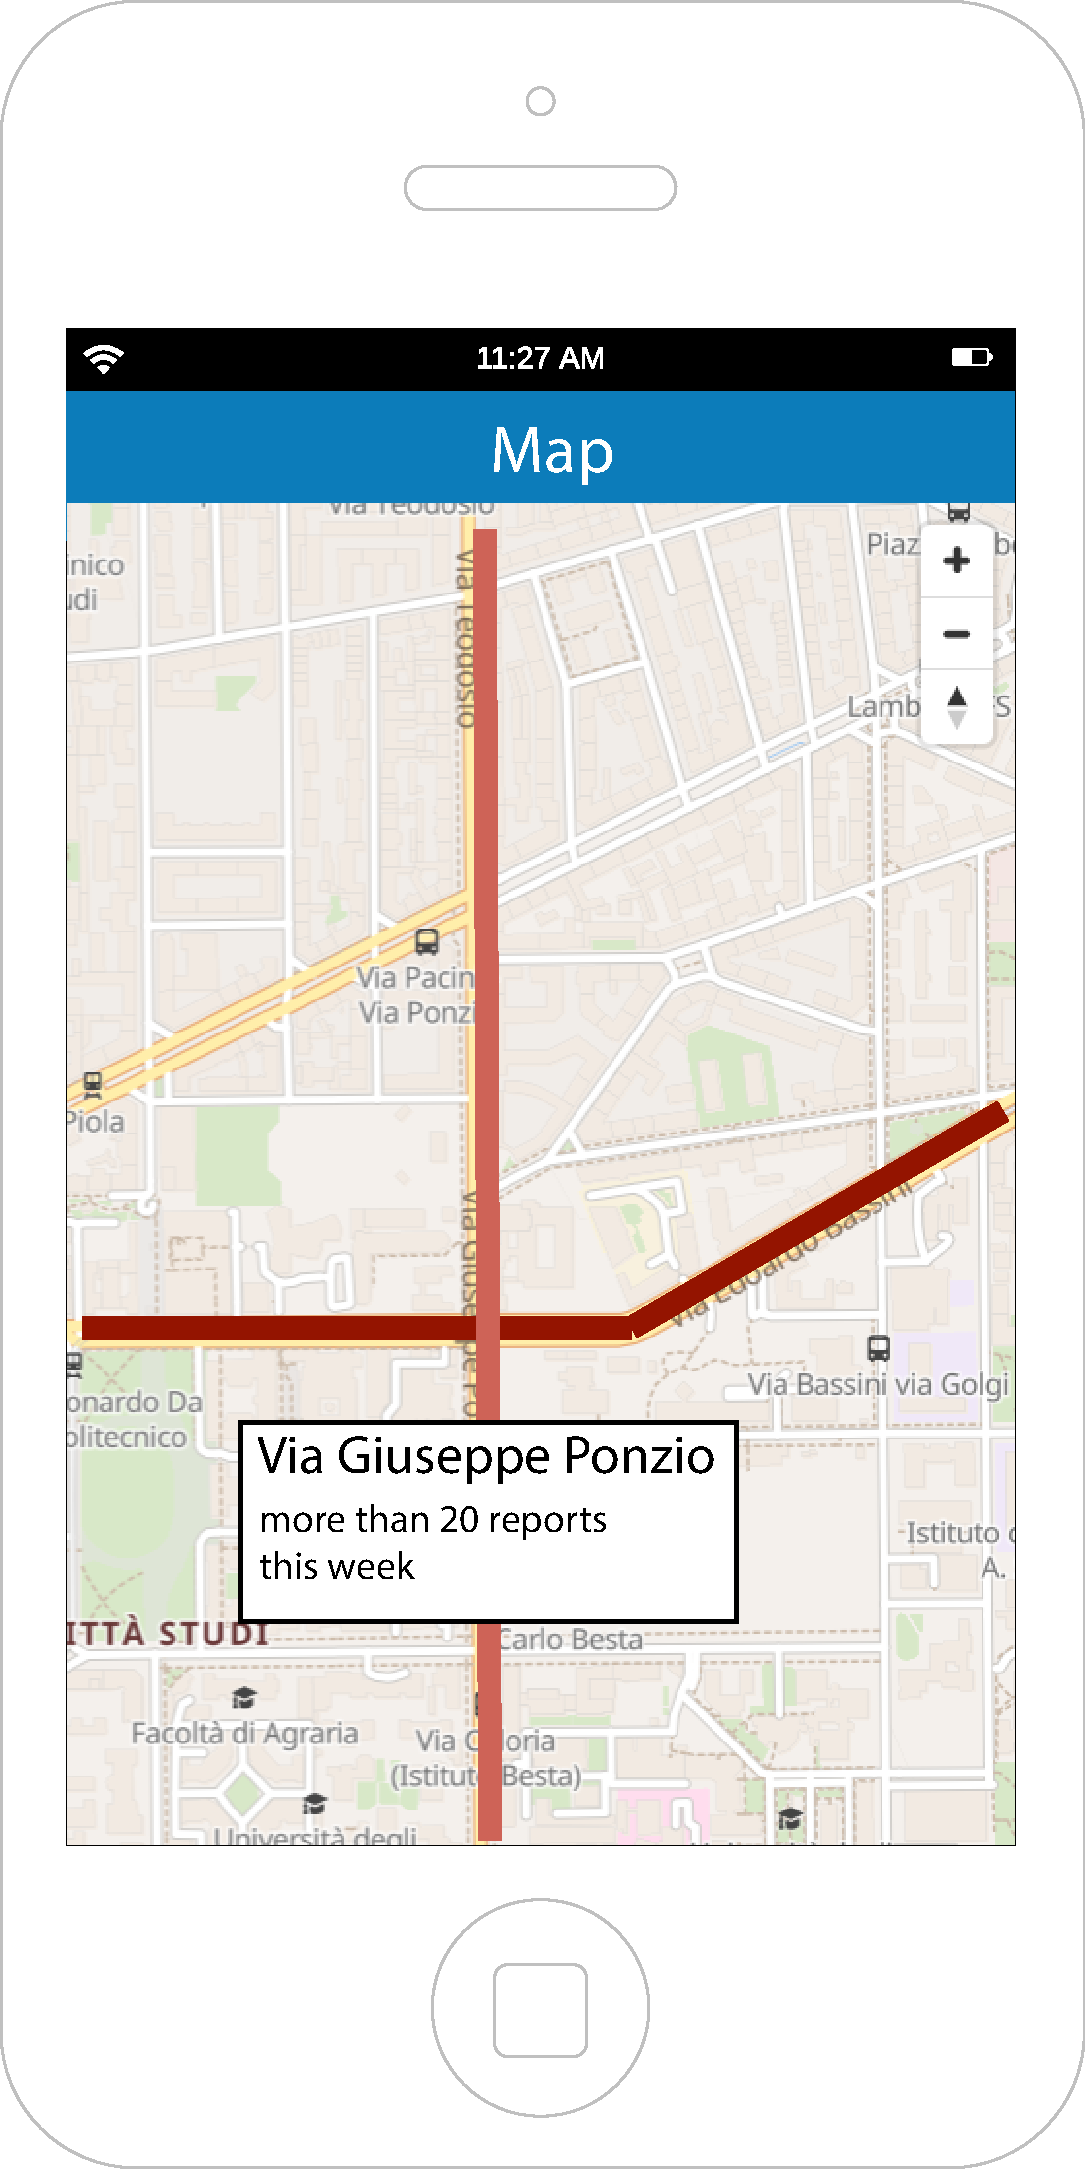
\includegraphics[scale=0.25, center]{Map-detail}
			\caption{User -  map detail}
			\label{fig:subim2}
		\end{subfigure}
		\end{figure}



		\begin{figure}[H]
		\begin{subfigure}{0.5\textwidth}
		\setcounter{subfigure}{6}
			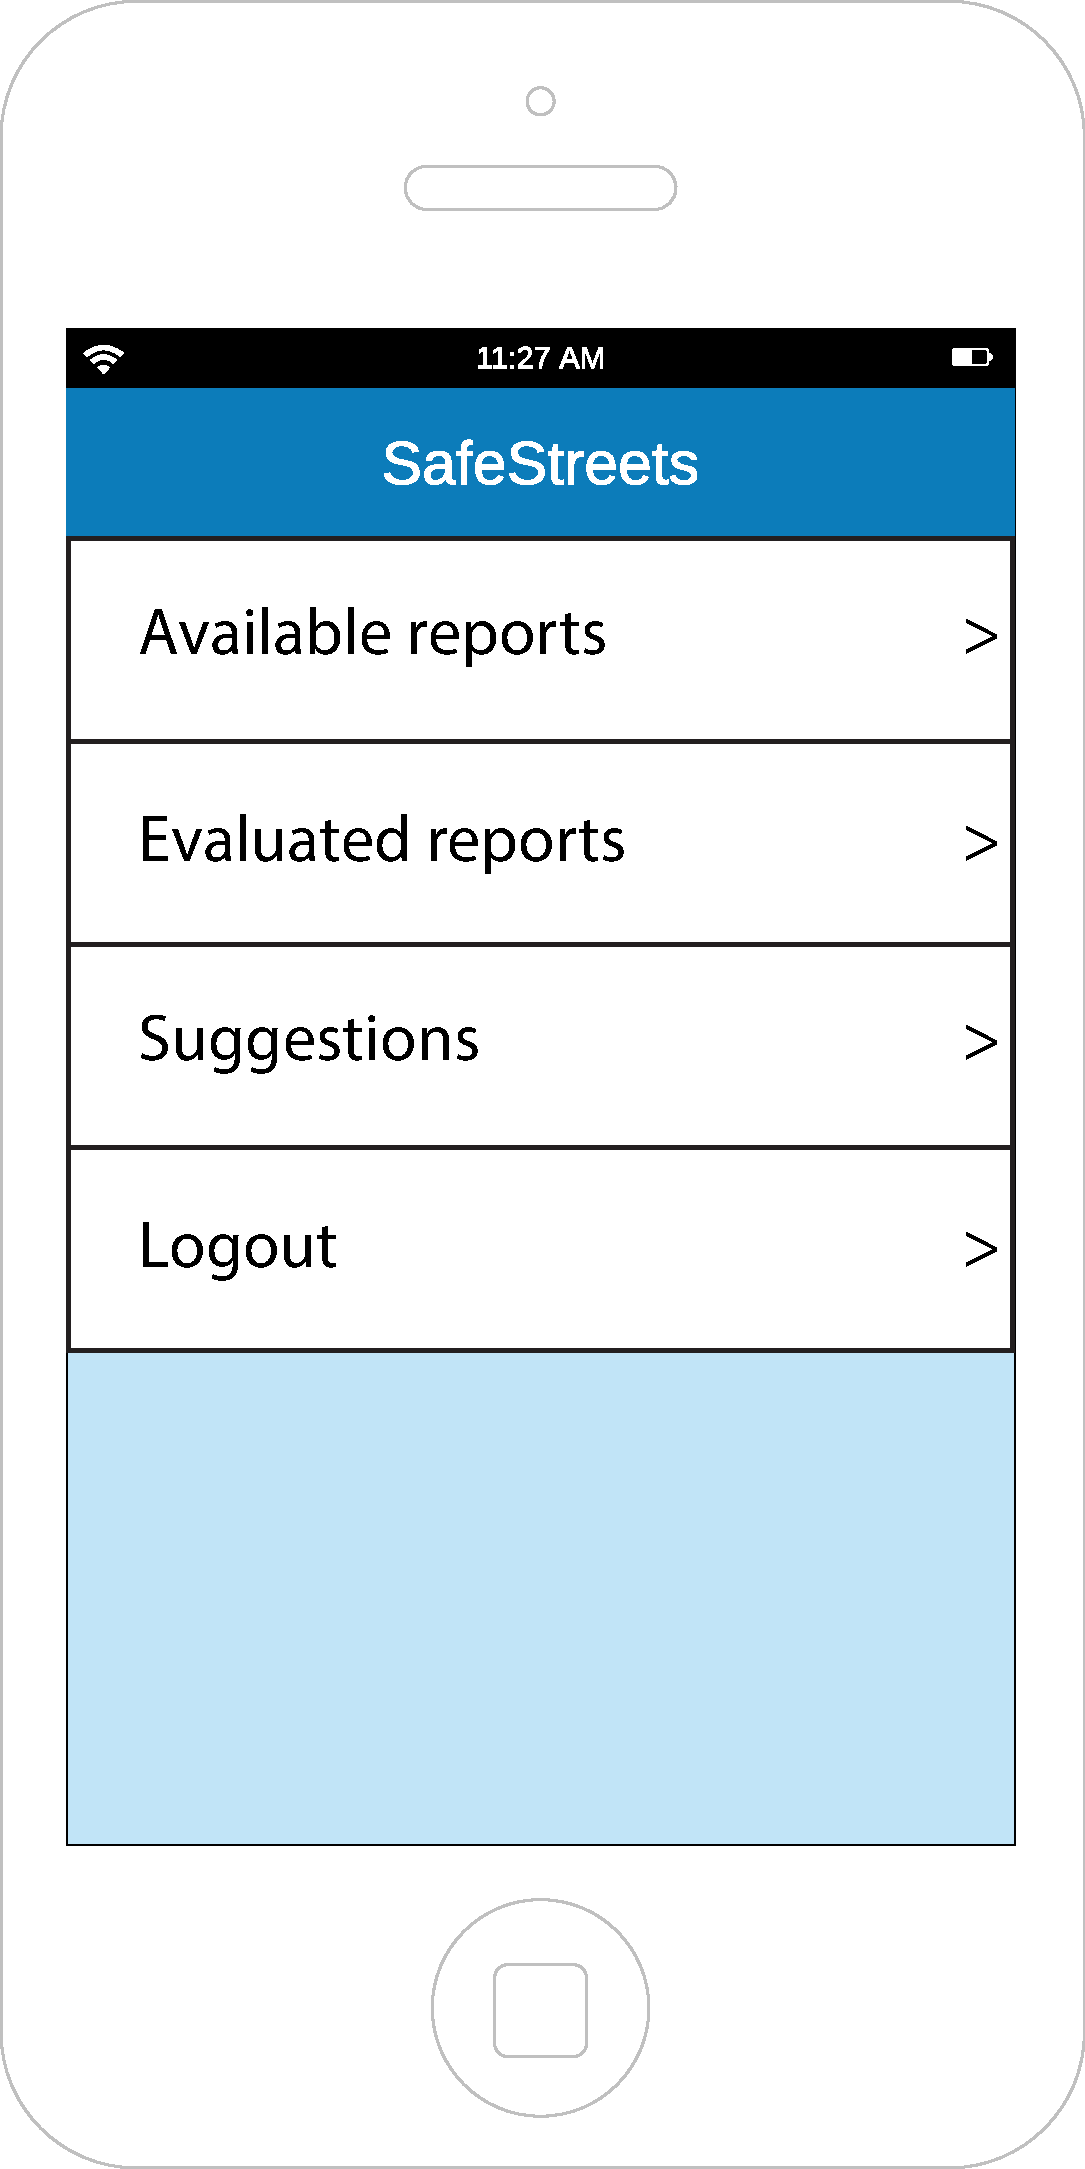
\includegraphics[scale=0.25, center]{HomeAut}
			\caption{Authority - home}
			\label{Authority - home}
		\end{subfigure}
		\begin{subfigure}{0.5\textwidth}
			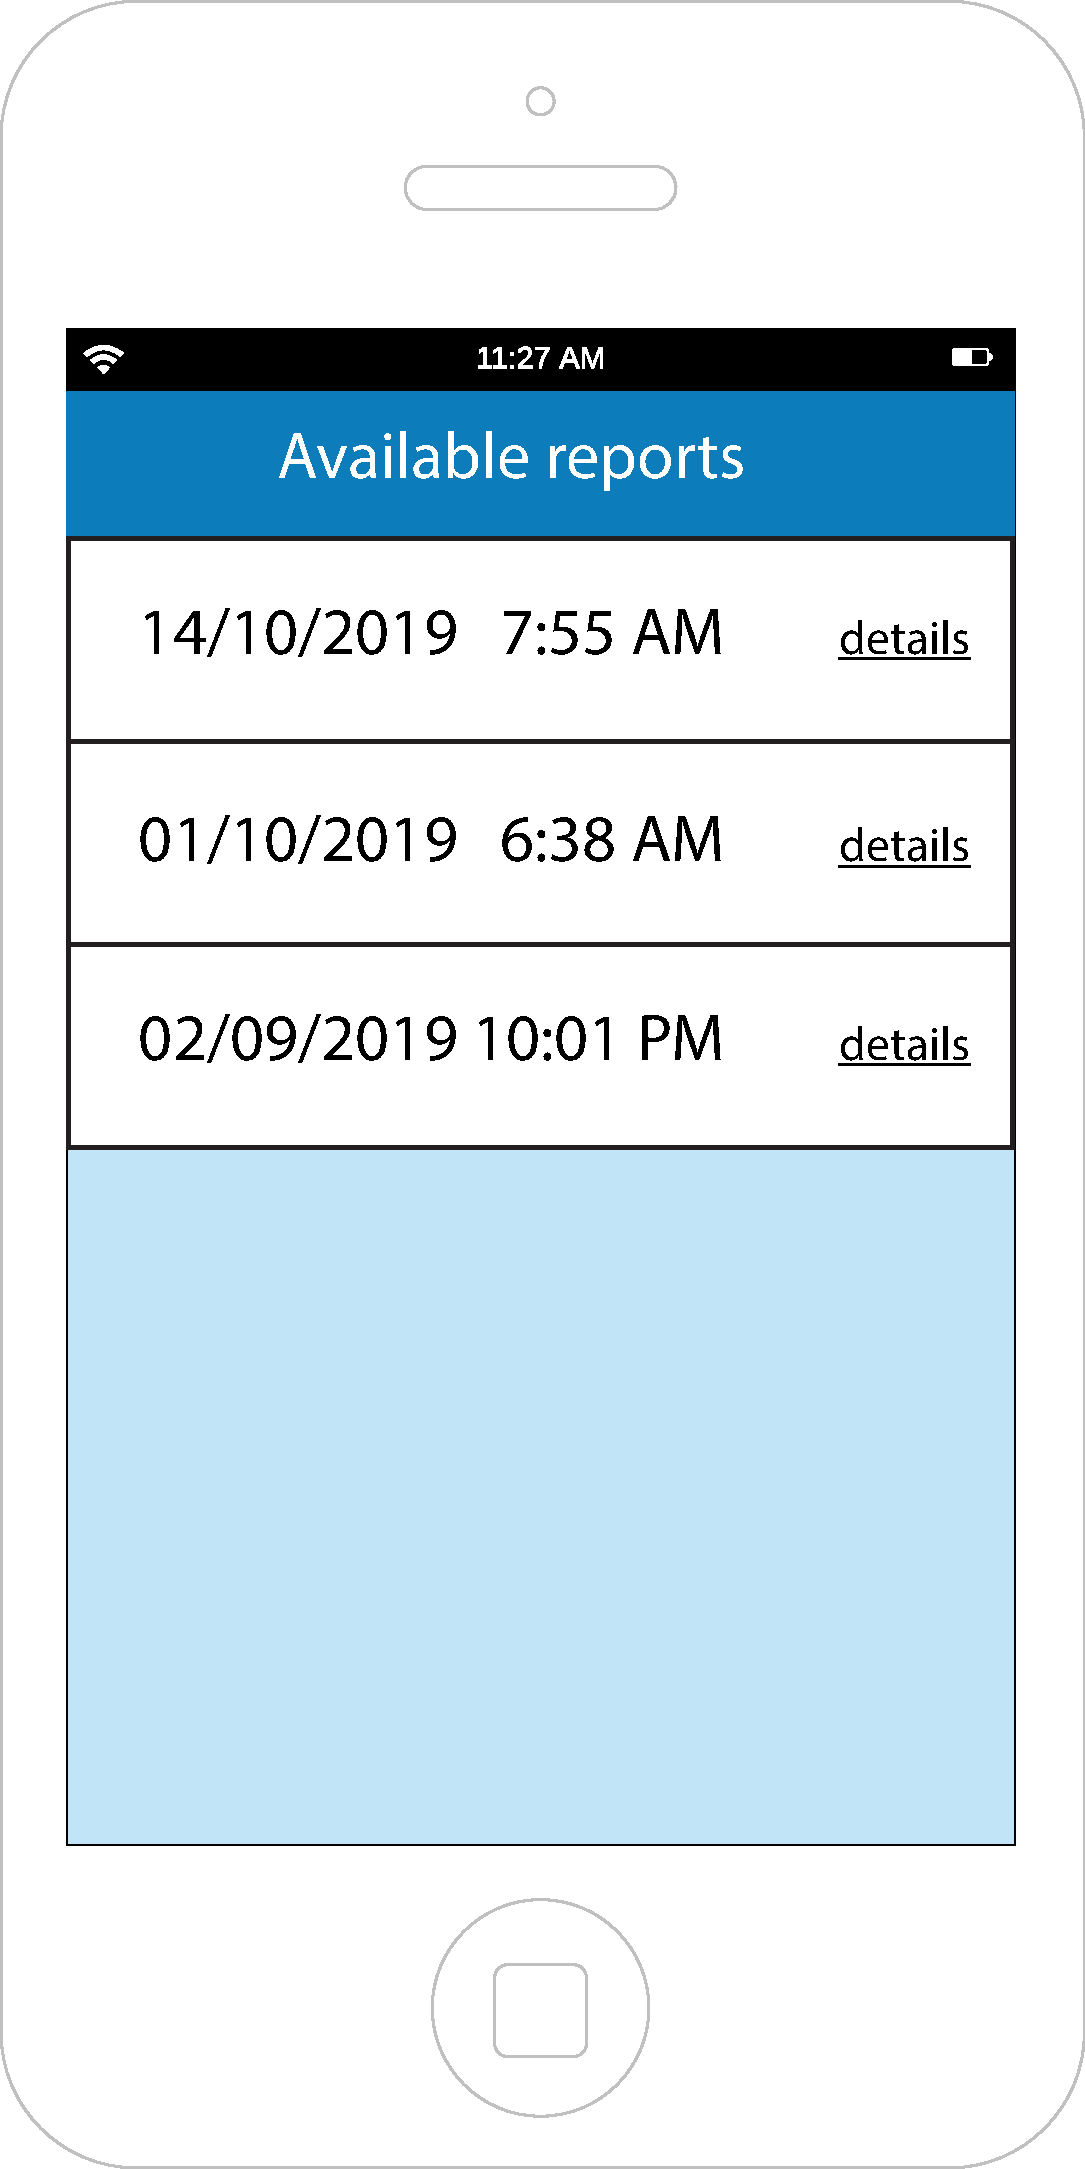
\includegraphics[scale=0.25, center]{Availablereports}
			\caption{Authority - available reports}
			\label{Authority - available reports}
		\end{subfigure}
		\end{figure}
		\begin{figure}[H]
		\begin{subfigure}{0.5\textwidth}
		\setcounter{subfigure}{8}
			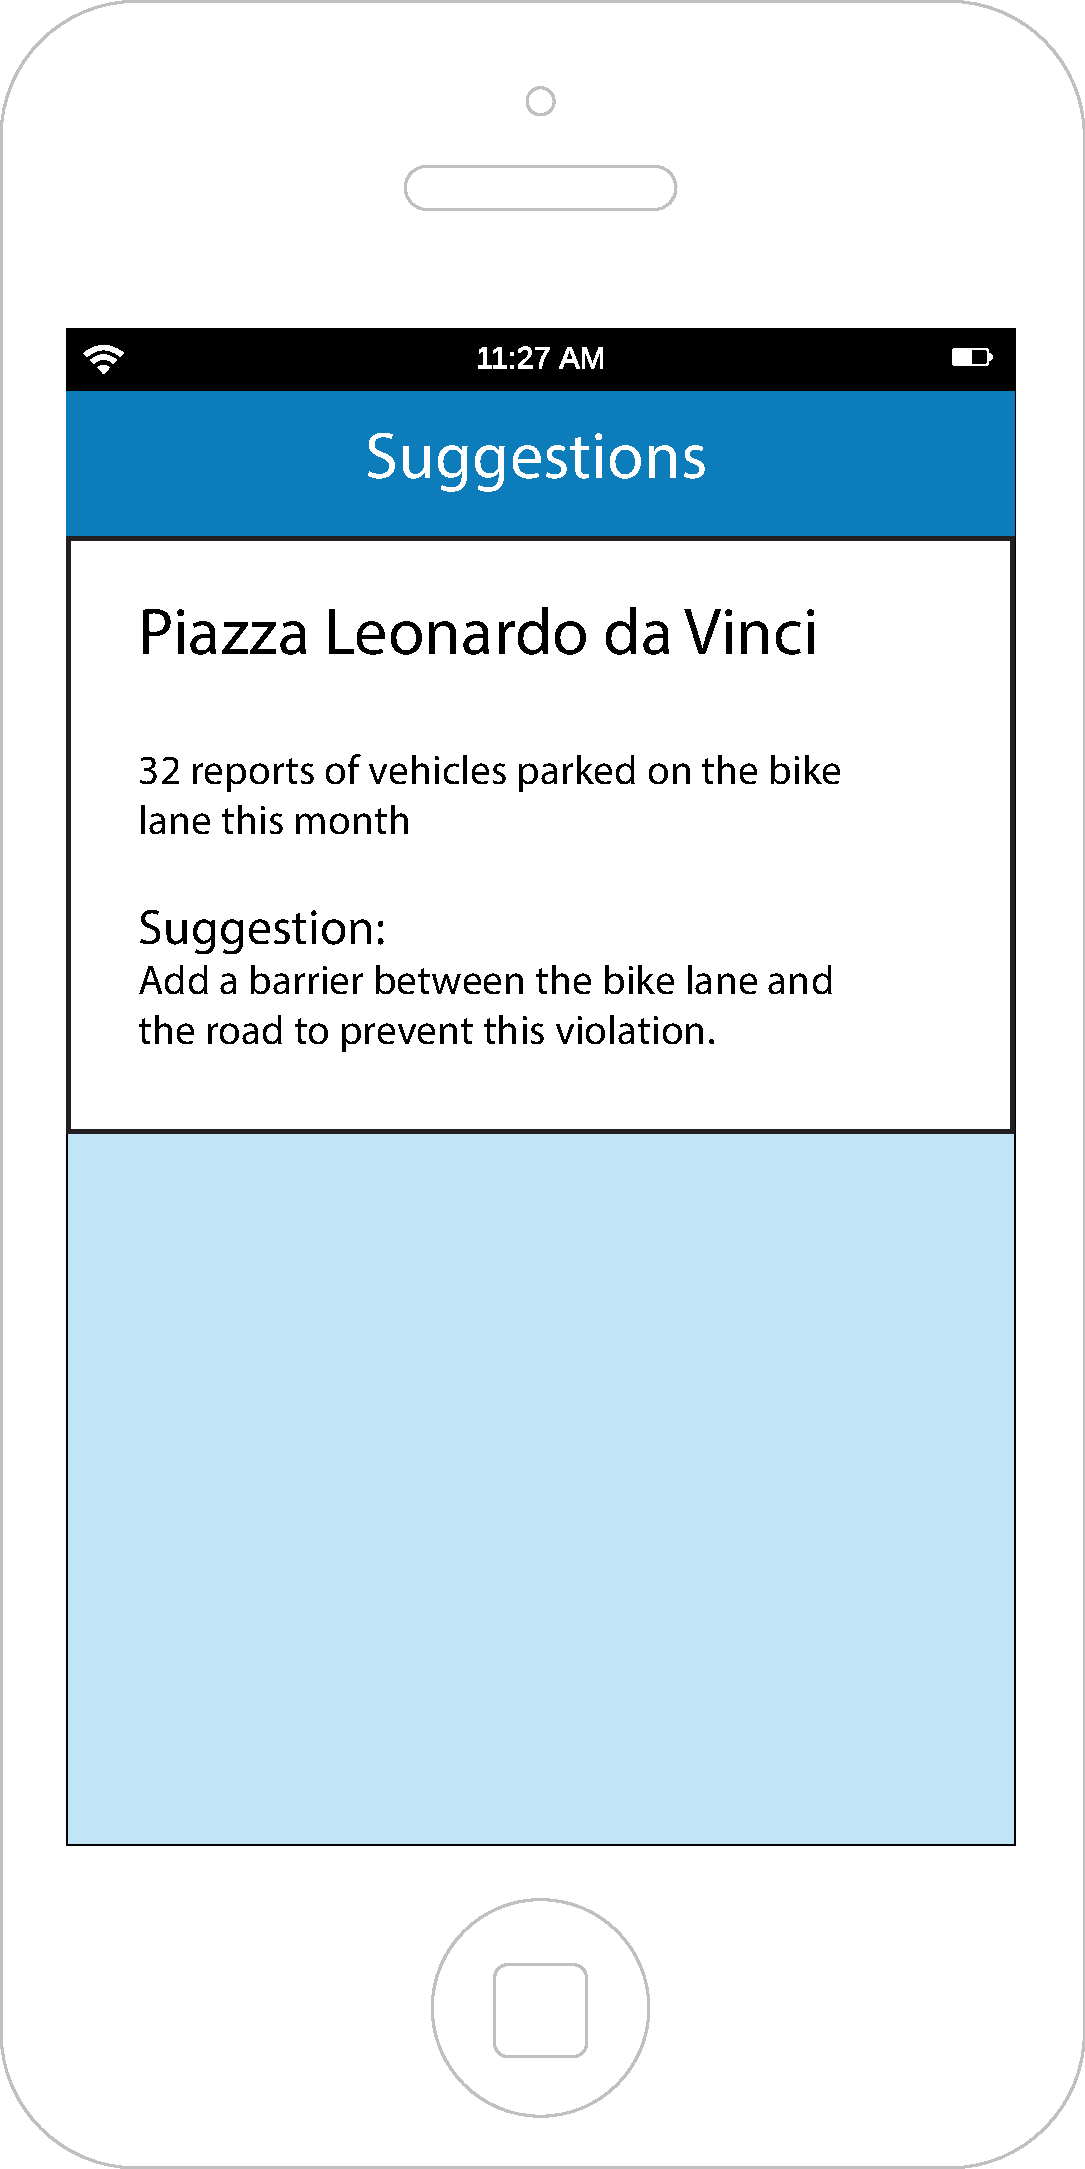
\includegraphics[scale=0.25, center]{Mysuggestions}
			\caption{Authority - suggestion}
			\label{Authority - suggestion}
		\end{subfigure}
		\begin{subfigure}{0.5\textwidth}
			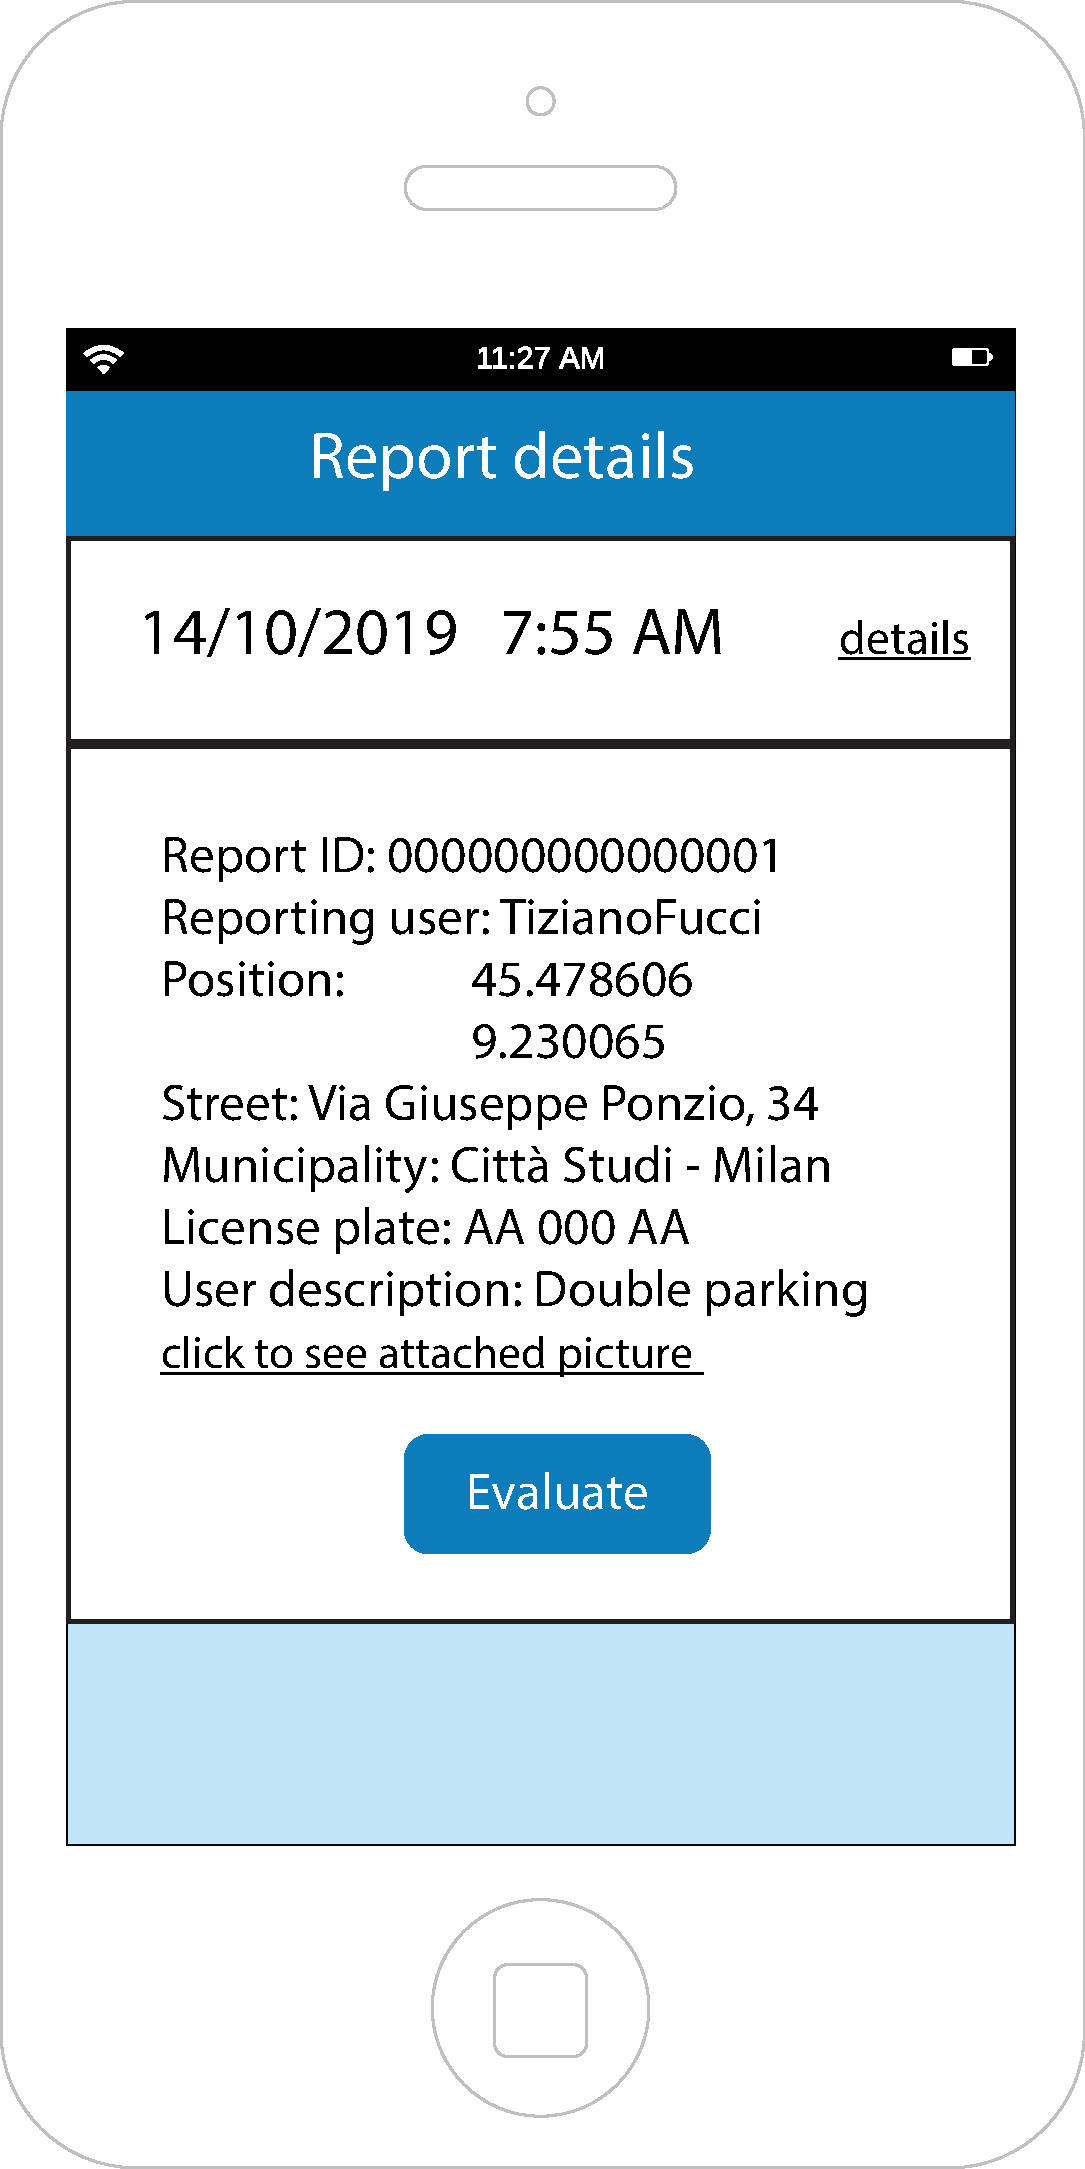
\includegraphics[scale=0.25, center]{Reportdetails}
			\caption{Authority - report details}
			\label{Authority - report details}
		\end{subfigure}
		\end{figure}
		

		\subsection{Hardware interfaces}
			The system has no hardware interfaces.
		\subsection{Software interfaces}
			The system has no software interfaces.
		\subsection{Communication interfaces}
			The system has no communication interfaces.
	\section{Functional Requirements}
		This section presents the requirements to be satisfied to reach each goal, in addition to the domain assumptions that must stand. Notice that the
		most trivial requirements (e.g. "The system always work properly") are omitted, in order to simplify the description.
		\subsection{User} 

			\paragraph {G1:} The application must allow the users to register, entering an e-mail address and a password, and to log in.
			\begin{itemize}
				\item{[R1]:} Registration must be allowed only entering a valid e-mail address that is not already associated to an existing SafeStreets account.
				\item{[R2]:} Registration must be allowed only entering a password that satisfies the safety conditions.
				\item{[R3]:} The system must store the hash of every password, using a safe cryptographic hash function.
				\item{[R16]}: Login must be allowed only if both e-mail address and password are correct.
			\end{itemize}

			\paragraph {G2:} The application must allow the users to notify traffic violations, providing the type of violation and a picture of the vehicle.
			\begin{itemize}
				\item{[D1]:} The users always provide a picture that allows both the algorithm to read the license plate and the authority to identify the violation.
				\item{[D2]:} Every user is provided with a device capable to share the exact GPS position at any moment.
				\item{[D3]:} The name of the street where a violation occured is retrieved from the GPS position.
				\item{[D5]:} Date, time and street of the violation are automatically inferred by the application.
				\item{[D6]:} The user sends the report staying in the same place of the violation attached to the report.
		 		\item{[D7]:} The picture of the license plate is taken at the moment and shows the right car.
			\end{itemize}
			\begin{itemize}
				\item{[R4]:} The system must check if the location of the report belongs to some municipality exploiting SafeStreets.
				\item{[R5]:} The system must add the right date, time and street of the violation to the data provided by the user.
				\item{[R6]:} The system must correctly read the license plate given a picture attached to a report.
			\end{itemize}

			\paragraph {G3:} The application must be able to show to the users the streets and the vehicles with the highest frequency of violations.
			\begin{itemize}
				\item{[D3]:} The name of the street where a violation occured is retrieved from the GPS position.
				\item{[D4]:} Authorities never make mistakes in evaluating a report.
				\item{[D5]:} Reports are evaluated only one time.
			\end{itemize}
			\begin{itemize}
				\item{[R5]:} The system must add the right date, time and street of the violation to the data provided by the user.
				\item{[R7]:} The system must exploit Google Maps APIs to show to the user the map of the violations.
				\item{[R8]:} The system must show the right colors on the map, given the number of approved reports for each street.
				\item{[R9]:} When a license plate is recognized, the system must show the number of approved reports for that car.
				\item{[R10]:} If the same violation is reported twice, it counts only one time on the map.
			\end{itemize}
				\paragraph {G4:}  The application must allow the user to see all of his reports and their status.
			\begin{itemize}
				\item{[R5]:} The system must add the right date, time and street of the violation to the data provided by the user.
				\item{[R11]:} The system must assign to each report a unique identification number.
			\end{itemize}
			\paragraph {G5:} The system must notify the user when one of his reports is evaluated.
			\begin{itemize}
				\item{[D3]:} The name of the street where a violation occured is retrieved from the GPS position.
				\item{[D4]:} Authorities never make mistakes in evaluating a report.
				\item{[D5]:} Reports are evaluated only one time.
			\end{itemize}
			\begin{itemize}
				\item{[R5]:} The system must add the right date, time and street of the violation to the data provided by the user.
				\item{[R7]:} The system must exploit Google Maps APIs to show to the user the map of the violations.
				\item{[R8]:} The system must show the right colors on the map, given the number of approved reports for each street.
				\item{[R9]:} When a license plate is recognized, the system must show the number of approved reports for that car.
				\item{[R10]:} If the same violation is reported twice, it counts only one time on the map.
			\end{itemize}

\paragraph{Scenarios}

				\subparagraph{Scenario 1}
					Mario, an elderly person who has a reserved parking lot, always has to spend time looking for a free
					car park, because someone frequently steals the one reserved to him without being sanctioned by the
					authorities. With the help of SafeStreets, Mario can report the parking thief to authorities and verify
					that he gets sanctioned.
					
				\subparagraph{Scenario 2}
					Luigi uses very frequently SafeStreets, but he is not sure if what he is doing is considered by authorities.
					Thanks to SafeStreets' reports history, now he is certain about which reports has been useful and which ones
					were wrong.
					
				\subparagraph{Scenario 3}
					Giuseppe is collecting some data about traffic and traffic violations for a University project. To retrieve more
					information he uses the map offered by SafeStreets, in order to learn which zones are more affected by traffic violations.
					
				\begin{figure}[H]
					\begin{subfigure}{\textwidth}
						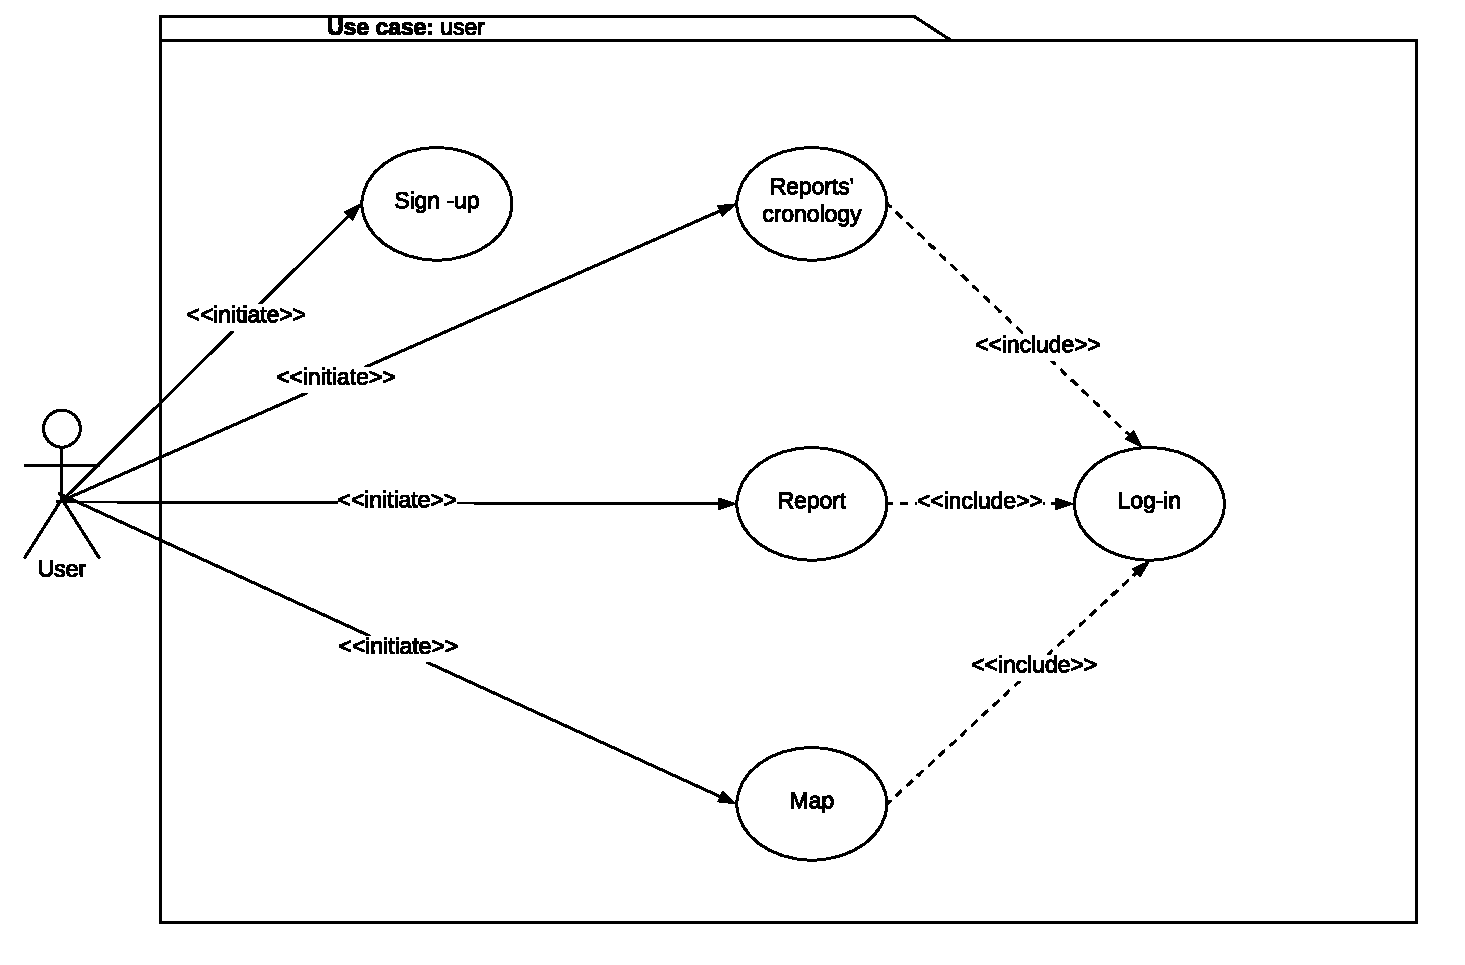
\includegraphics[scale = 0.75, center]{UseCaseC}
						\caption{State diagram on the behavior of reports for citizen}
					\end{subfigure}
				\end{figure}

				\begin{table}[H]
					\centering
					\begin{tabular}{|c|p{0.92\linewidth}|}
						\hline
						Name & {Sign up} \\
						\hline
						Actor & {User, Authorities} \\
						\hline
						Entry condition & {The User want to use for the first time SafeStreet and open the application on
									his device} \\
						\hline
						Events Flows &{ 
								\vskip 4pt
								\begin{enumerate}
									\item The user clicks on the ``Sign up" option
									\item The user fills all the mandatory fields
									\item The user agrees with the SafeStreet's privacy policy
									\item The user clicks on the confirmation option
									\item The system proceeds to verify user's data and to save them
								\end{enumerate}
								\vskip 4pt}\\
						\hline
						Exit Conditions & {The user is registered and the system has saved his data} \\
						\hline
						Exceptions & {
								\vskip 4pt
								\begin{itemize}
									\item The user has already signed up
									\item Username has been already used. In this case the System notify the user and
										suggests some free Usernames.
									\item The data were not correct. In this case the system ask to the user to check and
										correct eventual mistakes.
									\item Not all the mandatory fields were filled. In this case the system warns the user
										and notify him which fields are empty
								\end{itemize}
								\vskip 4pt
						} \\
						\hline
					\end{tabular}
					\caption{Sing up}
					\label{tab: }
				\end{table}

				\begin{table}[H]
					\centering
					\begin{tabular}{|c|p{0.92\linewidth}|}
						\hline
						Name & {Log in} \\
						\hline
						Actor & {User, Authorities} \\
						\hline
						Entry condition & {The User open the application because he want to access the service he 
									already signed up} \\
						\hline
						Events Flows &{ 
								\vskip 4pt
								\begin{enumerate}
									\item The user clicks on the ``Log in" option
									\item The user fills all the Username and password fields
									\item The user clicks the confirmation option
									\item The system proceeds to verify user's data
									\item The user has free access to the service now
								\end{enumerate}
								\vskip 4pt}\\
						\hline
						Exit Conditions & {The user is logged} \\
						\hline
						Exceptions & {
								\vskip 4pt
								\begin{itemize}
									\item Password wrong
									\item Username wrong, in both case the system will ask to check and correct the 
										log-in information
								\end{itemize}
								\vskip 4pt
						} \\
						\hline
					\end{tabular}
					\caption{Log in}
					\label{tab: }
				\end{table}
				
				\begin{table}[H]
					\centering
					\begin{tabular}{|c|p{0.92\linewidth}|}
						\hline
						Name & {Report} \\
						\hline
						Actor & {User} \\
						\hline
						Entry condition & {The User wants to report a traffic violation, so he opens the application and logs in,
									then he chooses the ``report" option} \\
						\hline
						Events Flows &{ 
								\vskip 4pt
								\begin{enumerate}
									\item The User clicks on ``Report" option
									\item The User takes a photo of the violation and the license plate of vehicle
									\item The system tries to read the plate from the photo
									\item The user checks that the system recognized correctly the plate
									\item The user inserts the type of violation.
									\item The user clicks on ``send report".
									\item The system retrieves the device street, date and time to fill the last fields
										of the report
								\end{enumerate}
								\vskip 4pt}\\
						\hline
						Exit Conditions & {The user reported the violation} \\
						\hline
						Exceptions & {
								\vskip 4pt
								\begin{itemize}
									\item The vehicle has been already reported.
									\item The system cannot obtain the user's position.
									\item Not all the fields has been filled.
									\item There is no internet connection available.
								\end{itemize}
								\vskip 4pt
						} \\
						\hline
					\end{tabular}
					\caption{Report}
					\label{tab: }
				\end{table}

				\begin{table}[H]
					\centering
					\begin{tabular}{|c|p{0.92\linewidth}|}
						\hline
						Name & {Chronology} \\
						\hline
						Actor & {User} \\
						\hline
						Entry condition & {The User open and log in the SafeStreet application} \\
						\hline
						Events Flows &{ 
								\vskip 4pt
								\begin{enumerate}
									\item The user clicks on ``History" option
									\item The system searches and sends a recap of all the user's reports
									\item The user can check all his reports
								\end{enumerate}
								\vskip 4pt}\\
						\hline
						Exit Conditions & {The user clicks on ``Exit" option} \\
						\hline
						Exceptions & {
								\vskip 4pt
								\begin{itemize}
									\item The user has no reports.
									\item There is no internet connection available.
								\end{itemize}
								\vskip 4pt
						} \\
						\hline
					\end{tabular}
					\caption{Use case Chronology}
					\label{tab: }
				\end{table}
				
				\begin{table}[H]
					\centering
					\begin{tabular}{|c|p{0.92\linewidth}|}
						\hline
						Name & {Visualize Map} \\
						\hline
						Actor & {User} \\
						\hline
						Entry condition & {The User opens SafeStreets, logs in and chooses the ``Visualize Map" option} \\
						\hline
						Events Flows &{ 
								\vskip 4pt
								\begin{enumerate}
									\item The user clicks on ``Visualize Map"
									\item The system retrieves the device position and obtains information about
										the near streets' reports number to calculate their ``level" and displays
										it correctly
									\item The user can navigate in the map seeing each street and their level
								\end{enumerate}
								\vskip 4pt}\\
						\hline
						Exit Conditions & {The user clicks on exit button} \\
						\hline
						Exceptions & {
								\vskip 4pt
								\begin{itemize}
									\item There is no internet connection
									\item The GPS system is not functioning
									\item The app doesn't have permits to access to device's position
								\end{itemize}
								\vskip 4pt
						} \\
						\hline
					\end{tabular}
					\caption{Use case on Visualize Map}
					\label{tab: }
				\end{table}
				
				\begin{figure}[H]
					\begin{subfigure}{\textwidth}
						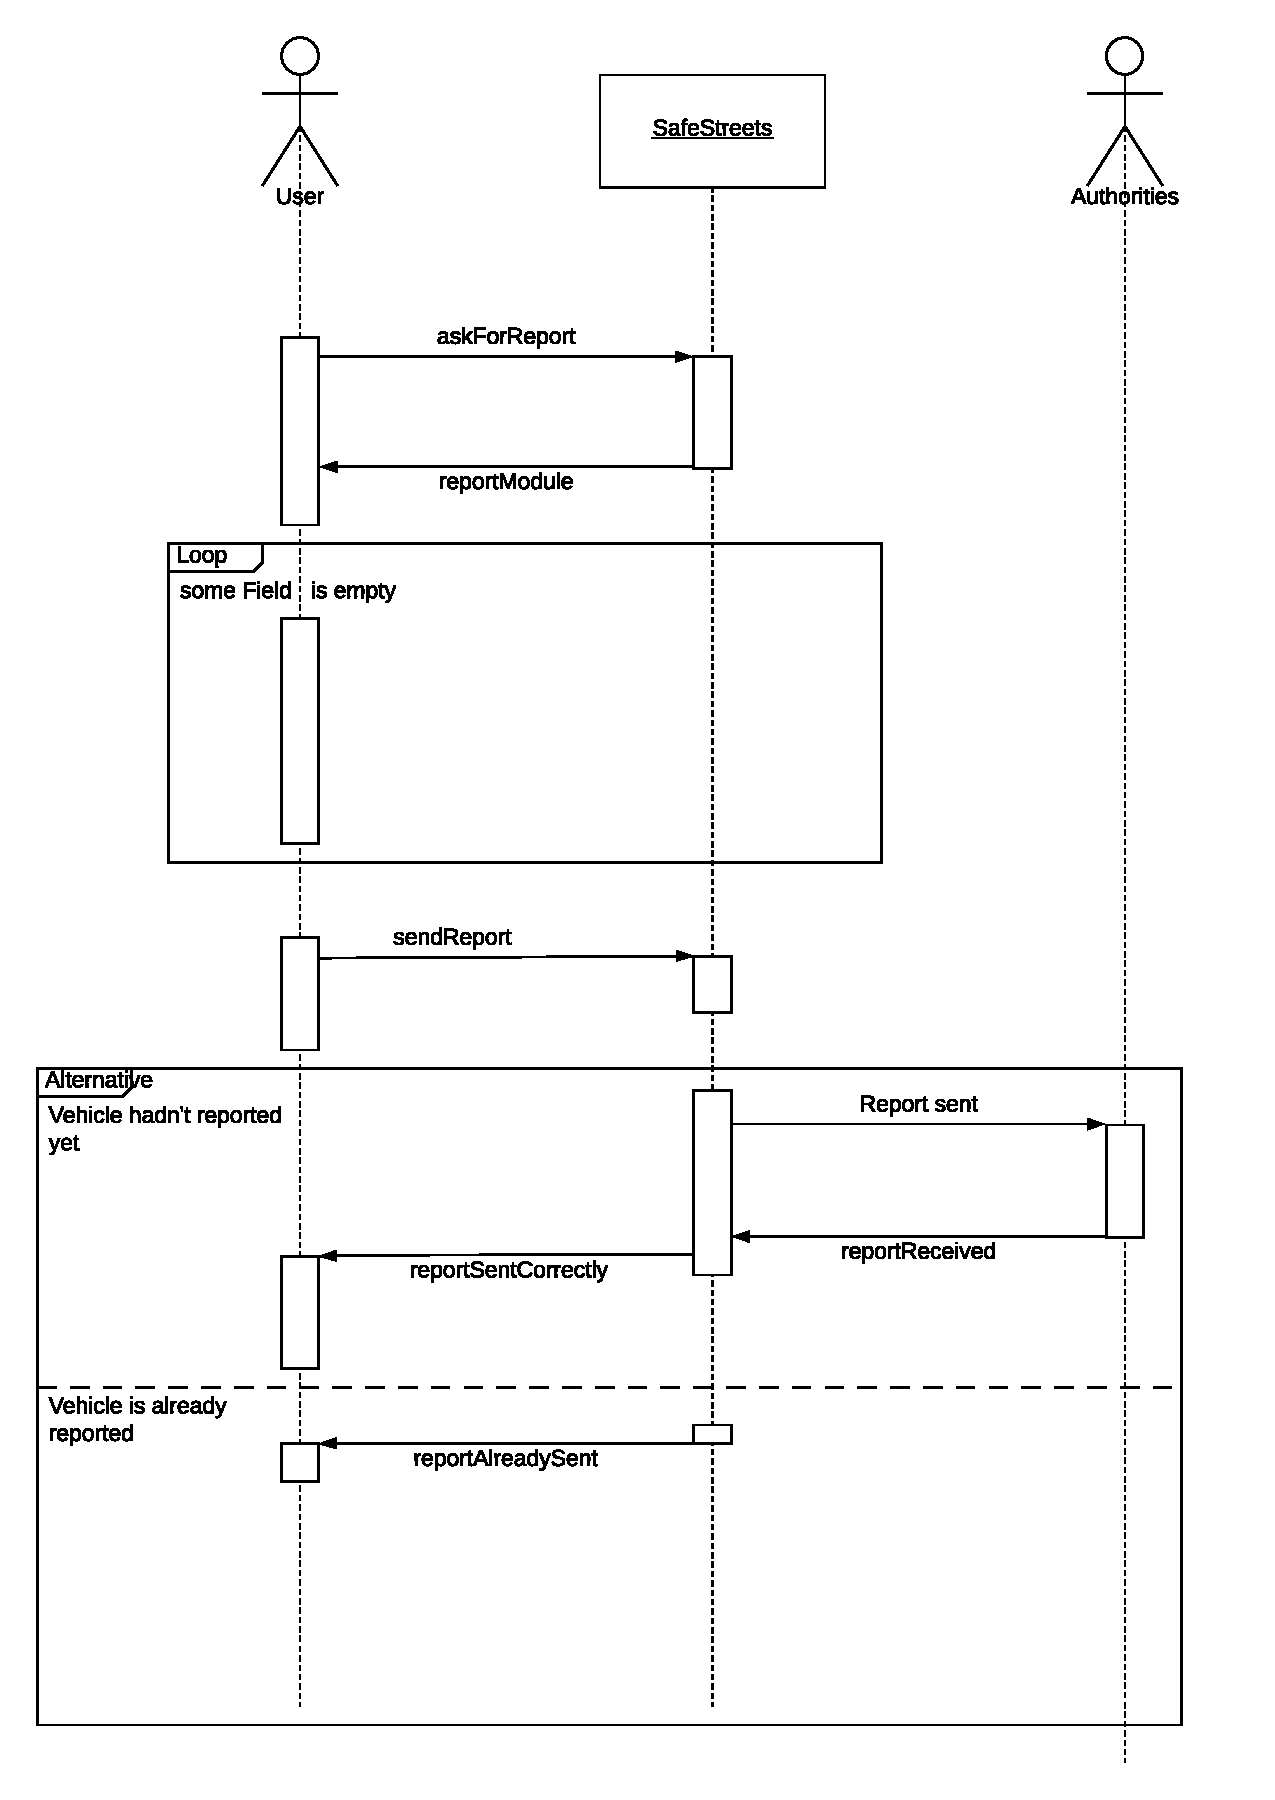
\includegraphics[scale = 0.75, center]{ReportSequenceDiagram}
						\caption{Sequence diagram on the behavior of reports for citizen}
					\end{subfigure}
				\end{figure}
				\begin{figure}[H]
					\begin{subfigure}{\textwidth}
						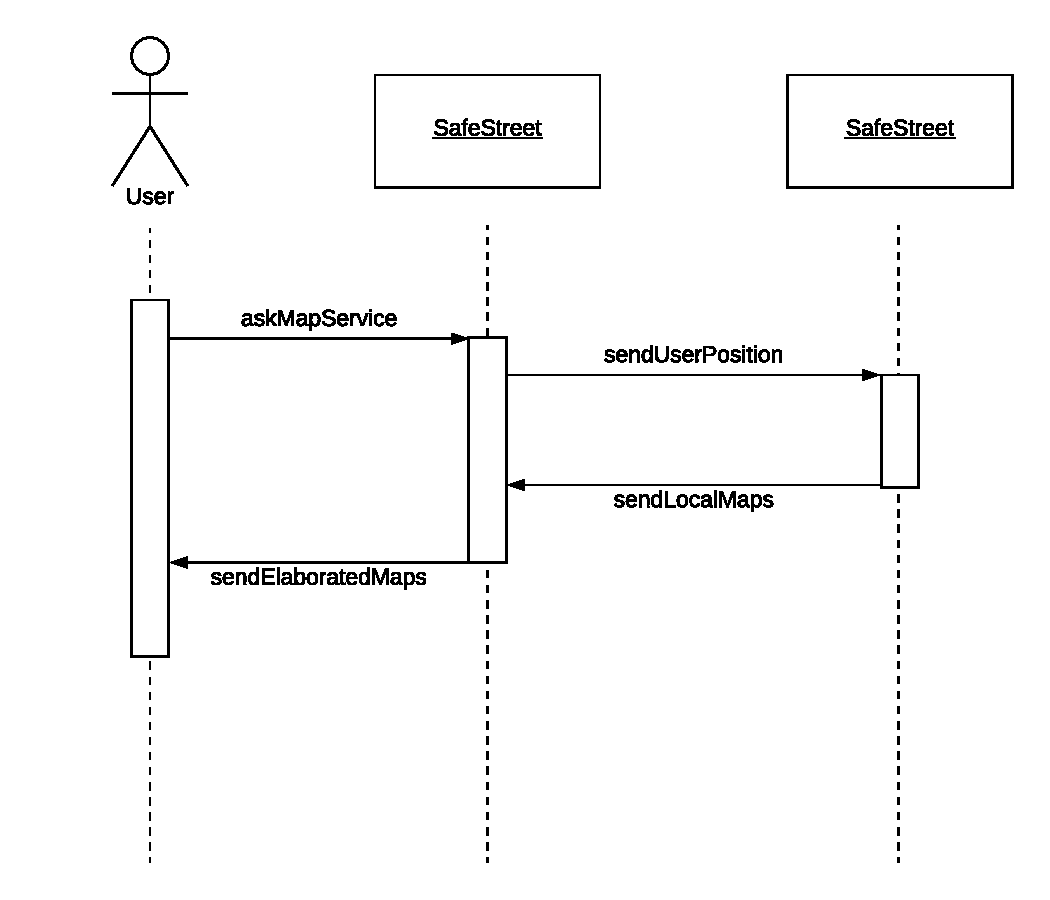
\includegraphics[scale = 0.70, center]{MapSequenceDiagram}
						\caption{Sequence diagram about Map option}
					\end{subfigure}
				\end{figure}
				\begin{figure}[H]
					\begin{subfigure}{\textwidth}
						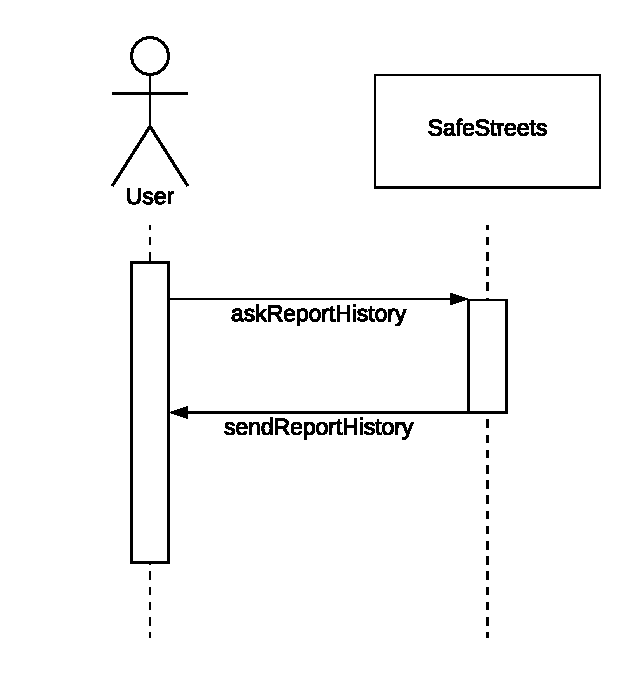
\includegraphics[scale = 0.70, center]{HhistorySequenceDiagram}
						\caption{Reports History}
					\end{subfigure}
				\end{figure}	
		\subsection{Authority}
			
			\paragraph {G6:} The application must allow the authorities to register, providing a valid identification number, a valid e-mail address and a valid password,
			and to log in.
				\begin{itemize}
					\item{[R1]:} Registration must be allowed only entering a valid e-mail address that is not already associated to an existing SafeStreets account.
					\item{[R2]:} Registration must be allowed only entering a password that satisfies the safety conditions.
					\item{[R3]:} The system must store the hash of every password, using a safe cryptographic hash function.
					\item{[R12]:} Registration must be allowed only entering a valid identification number that is not already associated to an existing SafeStreets account.
					\item{[R16]:} Login must be allowed only if both e-mail address and password are correct.
				\end{itemize}

			\paragraph {G7:} The application must allow authorities to retrieve and evaluate the available reports.
				\begin{itemize}
					\item{[D3]:} The name of the street where a violation occured is retrieved from the GPS position.
					\item{[D5]:} Reports are evaluated only one time.
				\end{itemize}
				\begin{itemize}
					\item{[R4]:} The system must check if the location of the report belongs to some municipality exploiting SafeStreets.
					\item{[R5]:} The system must add the right date, time and street of the violation to the data provided by the user.
					\item{[R11]:} The system must assign to each report a unique identification number.
					\item{[R13:]} The system must guarantee that each municipality is covered by at least one authority.
					\item{[R14]:} The system must notify the authorities when a new report is available.
				\end{itemize}
			\paragraph {G8:} The application must be able to identify potentially unsafe areas and suggest possible interventions.
				\begin{itemize}
					\item{[D3]:} Every user is provided with a device capable to share the exact GPS position at any moment.
			 		\item{[D4]:} Authorities never make mistakes in evaluating a report.
					\item{[D5]:} Date, time and street of the violation are automatically inferred by the application.
			 		\item{[D6]:} The user sends the report staying in the same place of the violation.
				\end{itemize}
				\begin{itemize}
					\item{[R10]:} If the same violation is reported twice, it counts only one time on the map.
					\item{[R13:]} The system must guarantee that each municipality is covered by at least one authority.
					\item{[R15]:} The system must suggest a possible intervention to the authorities of a municipality, according on the number of each type of violation.
				\end{itemize}

\paragraph{Scenarios}
				\subparagraph{Scenario 1}
					Eddie Edison, an officer, has noticed a vertiginous increment of traffic violations, so, to increase the control
					on the streets, he decides to join SafeStreets.
					
				\subparagraph{Scenario 2}
					Major Clancy Winchester has noticed that even with various tentatives to reduce the car accidents, he didn't
					succeed, so he decides to try to subscribe to and advanced option offered by SafeStreets trying to receive
					new suggestions to improve security.
					
				In this paragraph all the use cases diagram , use cases and sequence diagrams will be illustrated, the ``sign up" and ``log in"
				are not reported because are the same as above.

			
			\begin{figure}[H]
				\begin{subfigure}{\textwidth}
					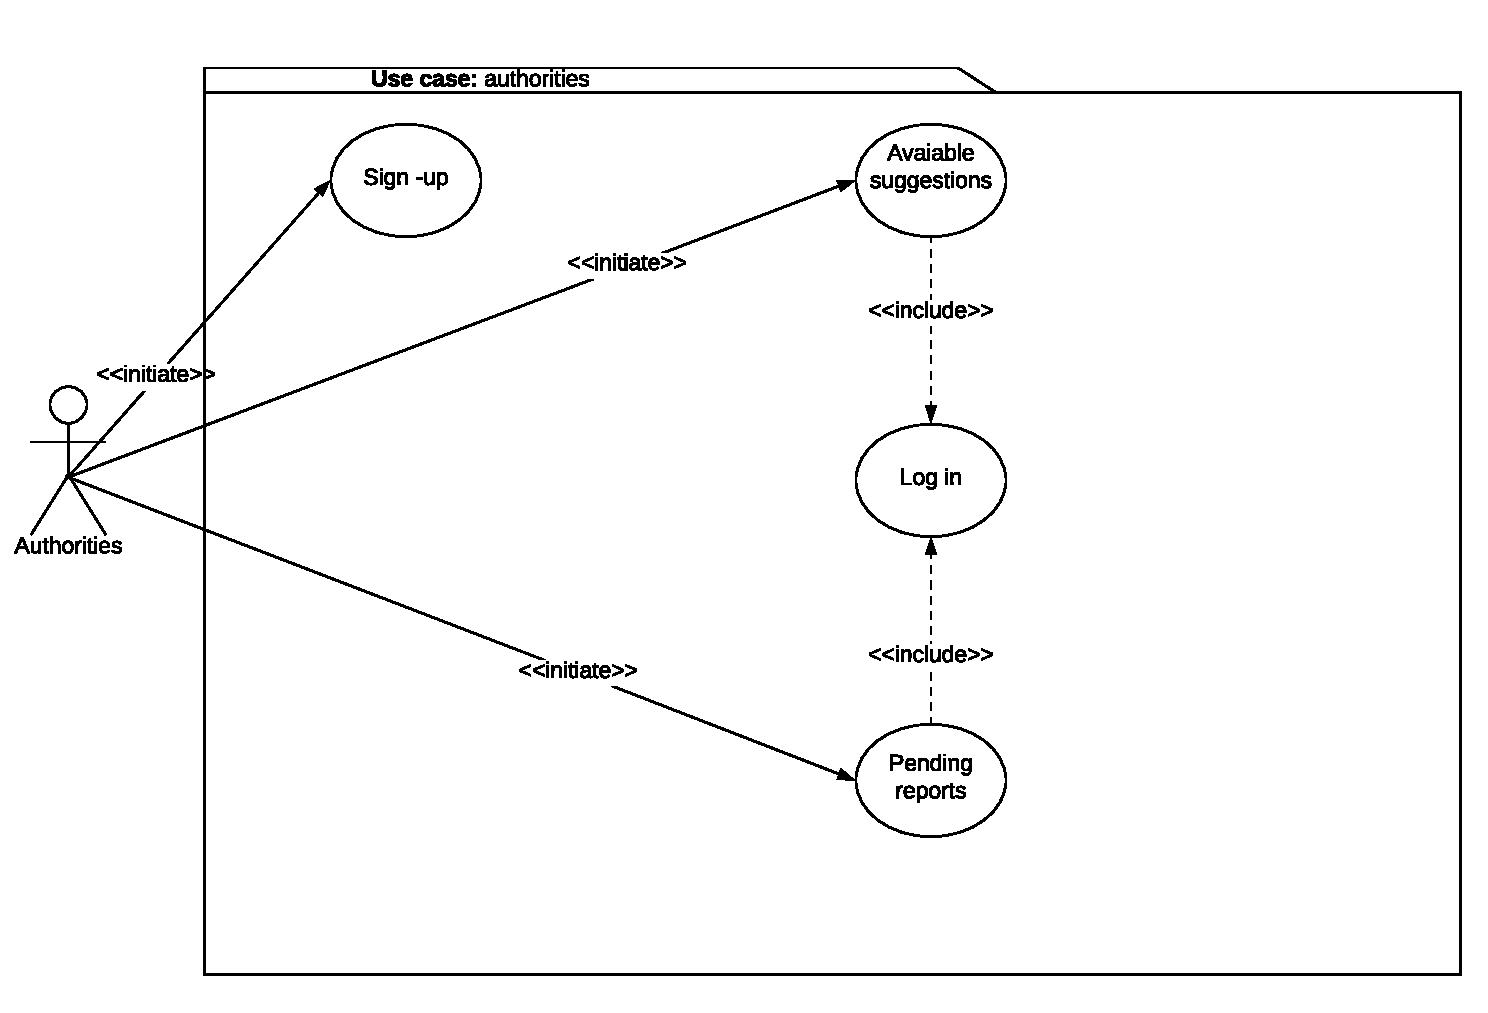
\includegraphics[scale = 0.75, center]{UseCaseA}
					\caption{Sequence diagram on the behavior of reports for users}
				\end{subfigure}
			\end{figure}
			

			\begin{table}[H]
				\centering
				\begin{tabular}{|c|p{0.92\linewidth}|}
					\hline
					Name & {Evaluate report} \\
					\hline
					Actor & {Authority} \\
					\hline
					Entry condition & {The authority is logged in} \\
					\hline
					Events Flows &{ 
							\vskip 4pt
							\begin{enumerate}
								\item The authority clicks on the ``Evaluate reports" options
								\item The system retrieves all the pending reports
								\item The authority chooses if accept or reject each single report based on the information
									contained in the report
							\end{enumerate}
							\vskip 4pt}\\
					\hline
					Exit Conditions & {The user clicks on exit button} \\
					\hline
					Exceptions & {/} \\
					\hline
				\end{tabular}
				\caption{Evaluate report}
				\label{tab: }
			\end{table}
			
			\begin{table}[H]
				\centering
				\begin{tabular}{|c|p{0.92\linewidth}|}
					\hline
					Name & {Suggestion} \\
					\hline
					Actor & {Authority} \\
					\hline
					Entry condition & {The authority is logged in} \\
					\hline
					Events Flows &{ 
							\vskip 4pt
							\begin{enumerate}
								\item The authority clicks on the ``Suggestion" option
								\item He chooses one Street under his control
								\item The system based on the street and the accidents gives a recommendation
							\end{enumerate}
							\vskip 4pt}\\
					\hline
					Exit Conditions & {The authority clicks on exit button} \\
					\hline
					Exceptions & {The authority hasn't activated this optional functionality} \\
					\hline
				\end{tabular}
				\caption{Evaluate report}
				\label{tab: }
			\end{table}
			
			\begin{figure}[H]
				\begin{subfigure}{\textwidth}
					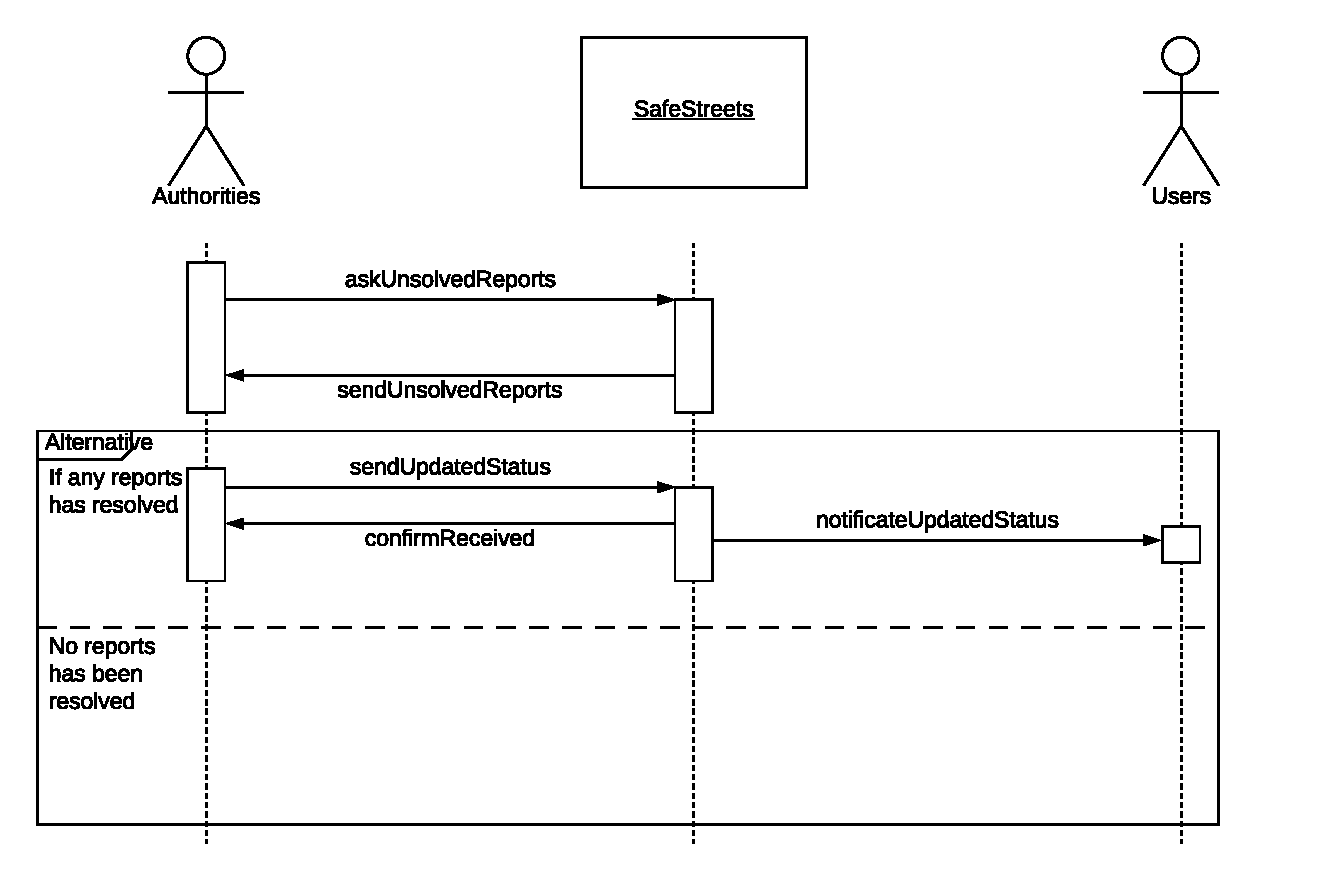
\includegraphics[scale = 0.75, center]{EvaluateSequenceDiagram}
					\caption{Sequence diagram on the behavior of reports for authorities}
				\end{subfigure}
			\end{figure}

			\begin{figure}[H]
				\begin{subfigure}{\textwidth}
					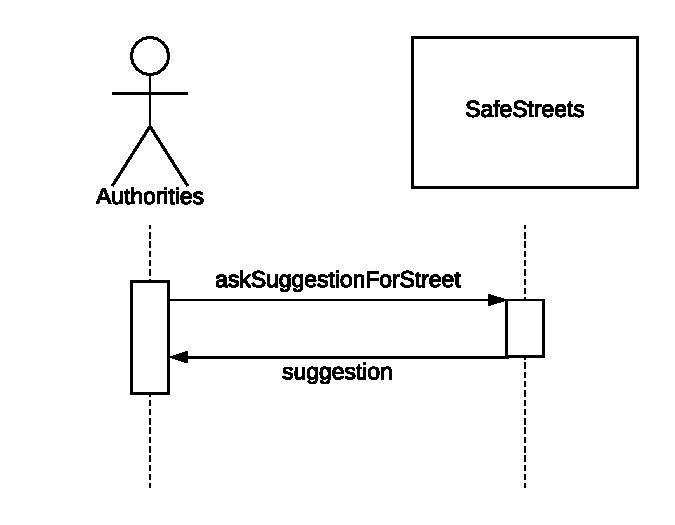
\includegraphics[scale = 0.75, center]{SuggestionSequenceDiagram}
					\caption{Sequence diagram on the behavior of reports for authorities}
				\end{subfigure}
			\end{figure}

	\subsection{World and Machine}
		In this subsection the World and Machine matrix is presented.
		\begin{table}[H]
			\centering
			\begin{tabular}{|c|c|c|}
				\hline
				Phenomenon & Shared & Who controls it\\
				\hline
				\hline
				Log-in & N & M\\
				\hline
				Sign-up & N & M\\
				\hline
				Someone made traffic violation & N & W\\
				\hline
				Report & Y & M\\
				\hline
				Visualize Map & N & M\\
				\hline
				Color on the map & N & M\\
				\hline
				Violations number & Y & W\\
				\hline
				Report Evaluated & Y & W\\
				\hline
				Notification received & N & M\\
				\hline
				Accident Occurs & N & W\\
				\hline
				A suggestion is made & N & M\\
				\hline
				
				
			\end{tabular}
			\caption{World and Machine matrix}
			\label{tab: }
		\end{table}
	
\newpage
	\subsection{Traceability Matrix}
			The following figure shows all the various requirements and use cases linking to each other.
			\begin{table}[H]
				\centering
				\begin{tabular}{|c|c|}
					\hline
					Requirement & Use Case \\ 
					\hline
					\hline
					R1 & \shortstack{\\Sign up \& Log in\\ Report} \\
					\hline
					R2 &  \shortstack{\\Sign up \& Log in\\ Report } \\
					\hline
					R3 &  \shortstack{\\Report} \\
					\hline
					R4 &  \shortstack{\\Visualize map} \\
					\hline
					R5 &  \shortstack{\\Visualize map} \\
					\hline
					R6 &  \shortstack{\\Report} \\
					\hline
					R7 &  \shortstack{\\Report} \\
					\hline
					R8 &  \shortstack{\\Sign up \&Log in} \\
					\hline
					R9 &  \shortstack{\\Reports \\Visualize Map} \\
					\hline
					R10 &  \shortstack{\\Reports \\ Evaluate report} \\
					\hline
					R11 &  \shortstack{\\Make suggestion} \\
					\hline
					R12 &  \shortstack{\\Report} \\
					\hline
				\end{tabular}
				\caption{Traceability matrix}
				\label{tab: }
			\end{table}



			
	
	\section{Performance Requirments}
		The System has to be able to serve a large number of users and authorities, simultaneously guaranteeing quick, 
		reactive and correct responses. It's important to underline that the accuracy of the suggestions received by the system
		are based on the data shared with SafeStreets and that the system does not guarantee that the proposed solution will surely
		solve the problem.
	\section{Design constraints}
		\subsection{Standards compliance}
			The error of the user's position is expressed in meters or feet (it depends on the unity preferred by the authorities) and has to be less than 10 meters.\\
			The system is designed to protect the privacy of users' data, as a matter of fact the entire 
			project is subject to the General Data Protection Regulation (GDPR), a regulation in EU 
			law on data protection and privacy for all individuals within the European Union (EU) and 
			the European Economic Area (EEA).
		\subsection{Hardware limitations}
			As specified in the ”dependencies and constraints” section, hardware requirements are present 
			only in relation to specific functionalities. For example, to make a report it is necessary a device with
			a functioning internet connection, a camera and a GPS sensor.\\
			So all the hardware requirements are:
			\begin{itemize}
				\item any type of Internet connection;
				\item a working gps sensor;
				\item a working camera.
			\end{itemize}
		\subsection{Any other costraint}
			The system does not have any other type of particular constraints. In order to protect users' privacy is important
			to remind that the data will be maintained secret (the authorities will not be able to see which user made a report)
			and that SafeStreets will respect the GDPR regulation.	\section{Software System Attributes}
		\subsection{Reliability}
			The system must be able to run continuously without any interruptions. In order to do that, it must 
			be ensured  that  the system is fault tolerant, this means that some precautions will be taken to avoid the system
			to be offline or unavailable. One of the many will be a daily backup of all the data on another server to avoid major
			data losses.
		\subsection{Availability}
			The system must have a fault tolerant architecture, the most important availability is about the reports and is supposed
			to be 99.999\%  of the time available (otherwise a huge number of reports could be lost and the system would never recover them). The other
			functionalities are supposed to be available 99.99\% of the time.
		\subsection{Security}
			The privacy is granted to both communication sides: the user doesn't know who evaluated his report and the authorities
			only see a number representing the user, so they cannot see any information like name or e mail. Confidentiality of client-server communication is granted exploiting PKC. The public key is used at the beginning of the session to exchange a secret symmetric key. The communication continues encrypting the messages with the symmetric key (e.g. an AES key). 
		\subsection{Maintainability}
			The system is realised with a modular structure, so it will be very easy to improve or substitute any part of it. For example, if one day a better recommender system is designed, the
			introduction of the new one will not impact the rest of the system.
		\subsection{Portablity}
			The application can be used on any mobile device respecting the hardware constraints.


	
% End of third chapter

\chapter{Formal Analysis}
	\section{Purpose}
This chapter shows the analysis of the Alloy model of the proposed system. Obviously, here the focus is only on some critical aspects of the application that require a special attention. In particular, the purpose of this model is to guarantee that:
\begin{itemize}
	\item The provided e-mail address is different for each user or authority;
	\item Every report has a unique identification number;
	\item Every municipality has at least one authority assigned;
	\item The authorities correctly receive notifications when a report is available;
	\item The users correctly receive notifications when one of their report is evaluated.
\end{itemize}

\newpage
	\section{Model}

	\lstinputlisting[language=alloy]{Model.als}

	\newpage

	\section{Results}
	The following is the result of the Alloy Analizer with the input shown in the previous section. 
		\begin{figure}[H]
				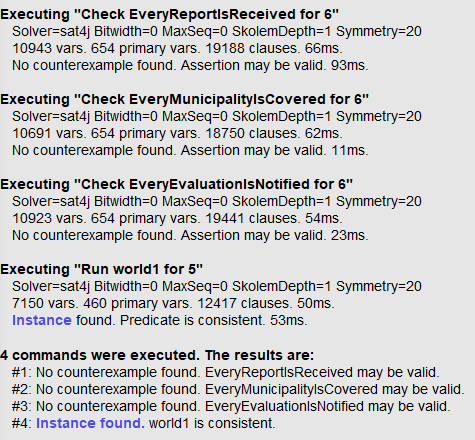
\includegraphics[scale = 0.9, center]{Consistency}
				\caption{Results}
		\end{figure}
	The \emph{world1} predicate is used to generate a world suitable to be read, which will be shown in the next section.
	

	\newpage

	\section{Generated world}
	Here is shown one of the possible worlds obtained by running \emph{world1}.


		\begin{figure}[H]
				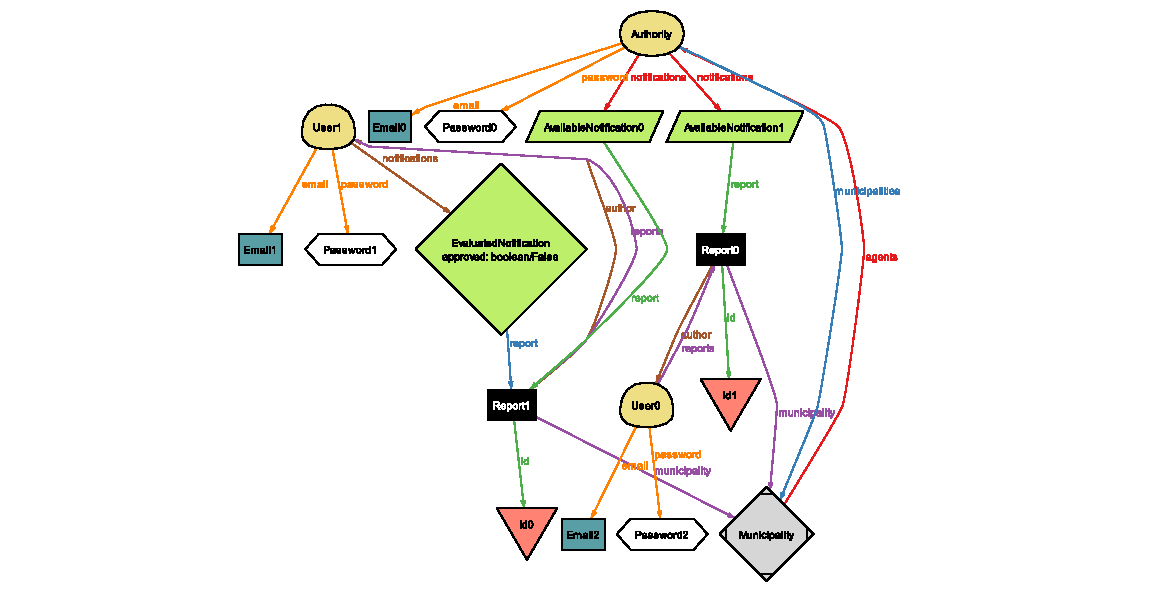
\includegraphics[scale = 1.4, center]{world1}				
				\caption{Generated world with two users, two reports}
		\end{figure}

	Of the two reports, only one has been evaluated and produced a notification that is correctly shown to the user. As said before, in the Alloy model every user has a different password, just to avoid arrows going all across the graph. 
% End of fourth chapter

\chapter{Effort Spent}
	\begin{table}[H]
		\centering
		\begin{tabular}{|c|c|c|}
			\hline
			Chapter & Frangi (hours) & Fucci (hours)\\
			\hline
			\hline
			Chapter 1 & 1 & 2\\
			\hline
			Chapter 2 & 7 & 4\\
			\hline
			Chapter 3 & 8 & 5\\
			\hline
			Chapter 4 & 2 & 8\\
			\hline
			Total hours: & 18 & 19\\
			\hline
		\end{tabular}
		\label{tab: }
	\end{table}
%End of fifth chapter

\chapter{References}

	\section{Bibliography}
	\begin{itemize}
	\item Course slides from Software Engineering 2 - \emph{Professor Elisabetta Di Nitto};
	\item 830-1998, IEEE Recommended Practice for Software Requirements Specifications - \emph{IEEE};
	\item 29148-2011, ISO/IEC/IEEE International Standard - Systems and software engineering - Life cycle processes - Requirements engineering - \emph{IEEE}.
	\end{itemize}

	\section{Tools}
	\begin{itemize}
	\item StarUML 3.1.0 - to draw and export UML diagrams;
	\item \url{lucidchart.com} - to draw, share and export state diagrams, sequence diagrams;
	\item Alloy Analizer 4.2 - to write and test the Alloy model of the application;
	\item Adobe Illustrator CC 2019 - to create mockups of the user interfeace;
	\item TeX Live 2019 - to write and organize this document;
	\item GitHub 2.23.0 - version control.
	\end{itemize}

% End of sixth chapter

\end{document}